\chapter{Energy-Harvesting Intermittent Systems} \label{chapter:review}

The emerging of energy harvesters provides diversified prospects for design paradigms of energy harvesting sensor nodes in IoT applications~\cite{miorandi2012internet}. This chapter first provides a review on various energy harvesting sources and corresponding energy harvesters in \sref{Section:EH}, followed by energy storage techniques that used in energy harvesting computing in \sref{Section:ES}. Energy-neutral computing, an early paradigm in energy harvesting computing, is reviewed in \sref{Section:EN}. Finally, two recent research topics towards storage-less energy harvesting computing, i.e. intermittent computing and power-neutral computing, are reviewed in \sref{Section:IC} and \sref{Section:PN} respectively with an illustration of proposed methodologies.

\section{Energy Harvesting Techniques} \label{Section:EH}
% how to relate this to my research

For all kinds of energy harvesters, although there is only one basic concept --- to extract energy from ambient sources, various energy sources and harvesters lead to miscellaneous output characteristics in the amount and wave forms of harvested power, voltage, and current. To select a energy harvester for powering sensor nodes, one important concern is whether the supply power level matches the consumption of the load~\cite{shaikh2016energy}. For one certain type of energy harvesters, the amount of energy harvesting supply can be scaled within an extent by the amount of energy sources or scaling the energy harvesters. The amount of energy sources is determined by the deploying environment, which cannot be controlled by the harvesting devices, but the size of energy harvesters can be decided at design-time with considerations on systems requirements, such as energy utilization, form factors, performance, etc. 
% On the other hand, to design sensor nodes that utilise one kind of energy harvesters, it is also necessary to match the power consumption of sensor nodes to the supply level. 

In order to appropriately size and designate energy harvesters for sensor nodes, the power features of different energy harvesters are widely considered by researchers and engineers~\cite{moss2015scaling}. A classification of common energy harvesting sources and corresponding energy harvesters used in IoT is presented in~\tref{Table:energysources}. The voltage and current features of different energy harvesters largely differ from each other, due to the intrinsic differences in temporal distributions of the available amount of different energy sources and the physical principles of power conversion. The following part of this section introduces each kind of energy sources and energy harvesting techniques listed in~\tref{Table:energysources}.
% , with their power features and current applications.
% power level/amount, features, variability

\begin{table}[!htb]
    \centering
    \begin{tabular}{|c|c|}
    \toprule
    \multirow{2}{*}{\textbf{Energy source}} & \multirow{2}{*}{\textbf{Energy harvester}} \\
     & \\ 
    \midrule
    Light & \multirow{2}{*}{Photovoltaic cells} \\
    (solar, artificial) & \\ 
    \midrule
    \multirow{2}{*}{Radio waves} & Radio frequency harvester \\ 
    & (antenna) \\ 
    \midrule
    Flow & Wind turbine, \\ 
    (air, liquid) & hydrogenerator \\ 
    \midrule
    Mechanical & Electromagnetic, electrostatic, \\ 
    (vibrations, pressure, stress-strain) & piezoelectric harvester \\ 
    \midrule
    \multirow{2}{*}{Heat} & \multirow{2}{*}{Theomo electric generator} \\
     & \\  
    \bottomrule
    \end{tabular}
    \caption{Classification of energy sources and energy harvesters in IoT.}
    \label{Table:energysources}
\end{table}

\subsection{Light Energy Harvesting}

Due to the abundant energy amount of light, whether from outdoor sunlight or indoor artificial light, light energy becomes a feasible source to powering sensor nodes and is historically treated as a substitute for battery supplies~\cite{raghunathan2005design, seah2009wireless}. Light energy can be converted to DC power by photovoltaic (PV) cells, which consist of semiconducting materials, e.g. silicon. When PV cells absorb light, electrons are excited by the photovoltaic effect, producing an electric potential by the separation of electrons and holes.

Given a fixed intensity of light, the output current from PV cells manifests an inverse relationship with the output voltage, as there is a semiconducting bypass within the PV cells. Although the power conversion efficiency may vary among different PV cell techniques (such as monocrystalline, polycrystalline, thin film), the curve shapes of current-voltage relationships are similar. Obviously, higher irradiance leads to higher current output when the output voltage is fixed, because there is more intensive light sources provided. More importantly, the output feature of PV cells can be summarised like "an inverse semiconductor" ------ when the terminal voltage is low, the output current is almost constant and close to short-circuit current; when the terminal voltage gets close to open-circuit voltage, the output current significantly decreases and finally terminates at the open-circuit voltage. 

Typical current-voltage curves of PV cells are shown in~\fref{Figure:solar_vi}, with an example of a monocrystalline cell given five values of illumination intensity from 200 W/m$^{2}$ to 1000 W/m$^{2}$. When the voltage is under 15V, the PV cell is similar to a current generator (so when the voltage increases, the power increases almost linearly). When the output voltage increases above 15V, the output current drops significantly and reaches zero at around 22V. According to this phenomenon, there is a voltage point where the cell produces the maximum power, which is named Maximum Power Point (MPP) as indicated by black dots in~\fref{Figure:solar_vi}. 

\begin{figure}[!htb]
    \centering
    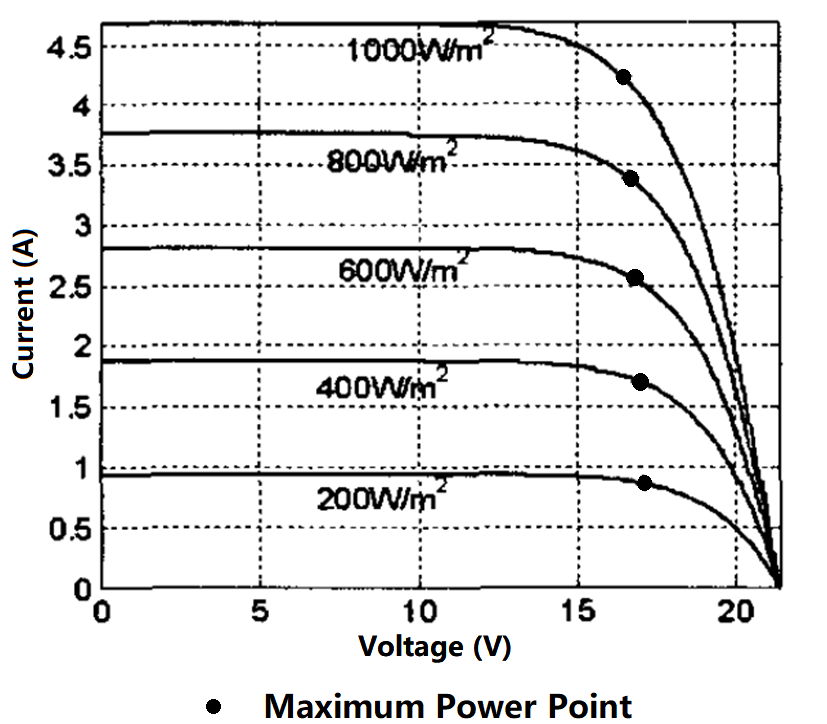
\includegraphics[width=10cm]{ch2_review/figures/solar_vi}
    \caption{Typical current-voltage curve of a solar module (monocrystalline, adapted from~\cite{xiao2004novel})}
    \label{Figure:solar_vi}
\end{figure}
% This figure is rubbish, can you replace it with a better one if possible!!!!!

In order to extract as much power as possible out of PV panels, most energy harvesting systems with PV modules adopts maximum power point tracking (MPPT) techniques~\cite{lopez2010new, paz2016high, verma2016maximum}. MPPT is achieved by dynamically controlling the output voltage of PV cells around the maximum power point (MPP).
% When the energy harvester and the energy storage are directly coupled, the operating voltage, which is decided by the charges stored in the energy storage, is usually not at the MPP. However, adopting MPPT circuits inevitably costs energy and reduces the energy efficiency of the whole system. 

Outdoor sunlight and indoor artificial light are two main sources for light energy harvesting. The illumination intensity of direct sunlight on the earth's surface is typically 1000 $W/m^2$~\cite{roundy2004power}, while the typical indoor illumination intensity is 10 $W/m^2$~\cite{shaikh2016energy}. Due to this large difference in the power density of these two circumstances, PV modules are more prospective in outdoor applications for harvesting solar energy. Conversion efficiency of PV cells is typically 15\% to 25\% in outdoor conditions~\cite{mathuna2008energy}.  

Solar energy is an uncontrollable but partially predictable source~\cite{heinemann2006forecasting, buchli2014dynamic}. Solar irradiance demonstrates daily and annual periodicity due to the regularity of celestial movements, as well as irregular variations due to cloud movements, air mass, etc. A 3-year trace of diurnal global horizontal solar energy available measured in Los Angeles from 2012 to 2014 is presented in~\fref{Figure:solar_calendar}, and an example of daily dynamics of global horizontal solar irradiance of the same location is presented in~\fref{Figure:solar_plots}. As shown in both figures, the predictability is reflected from the roughly annual and daily periodicity, and the uncontrollability and randomness relates to the irregular variations, which include both daily variations in an annual scale and variations over a few seconds and minutes on a daily scale. 

\begin{figure}[!htb]
    \centering
    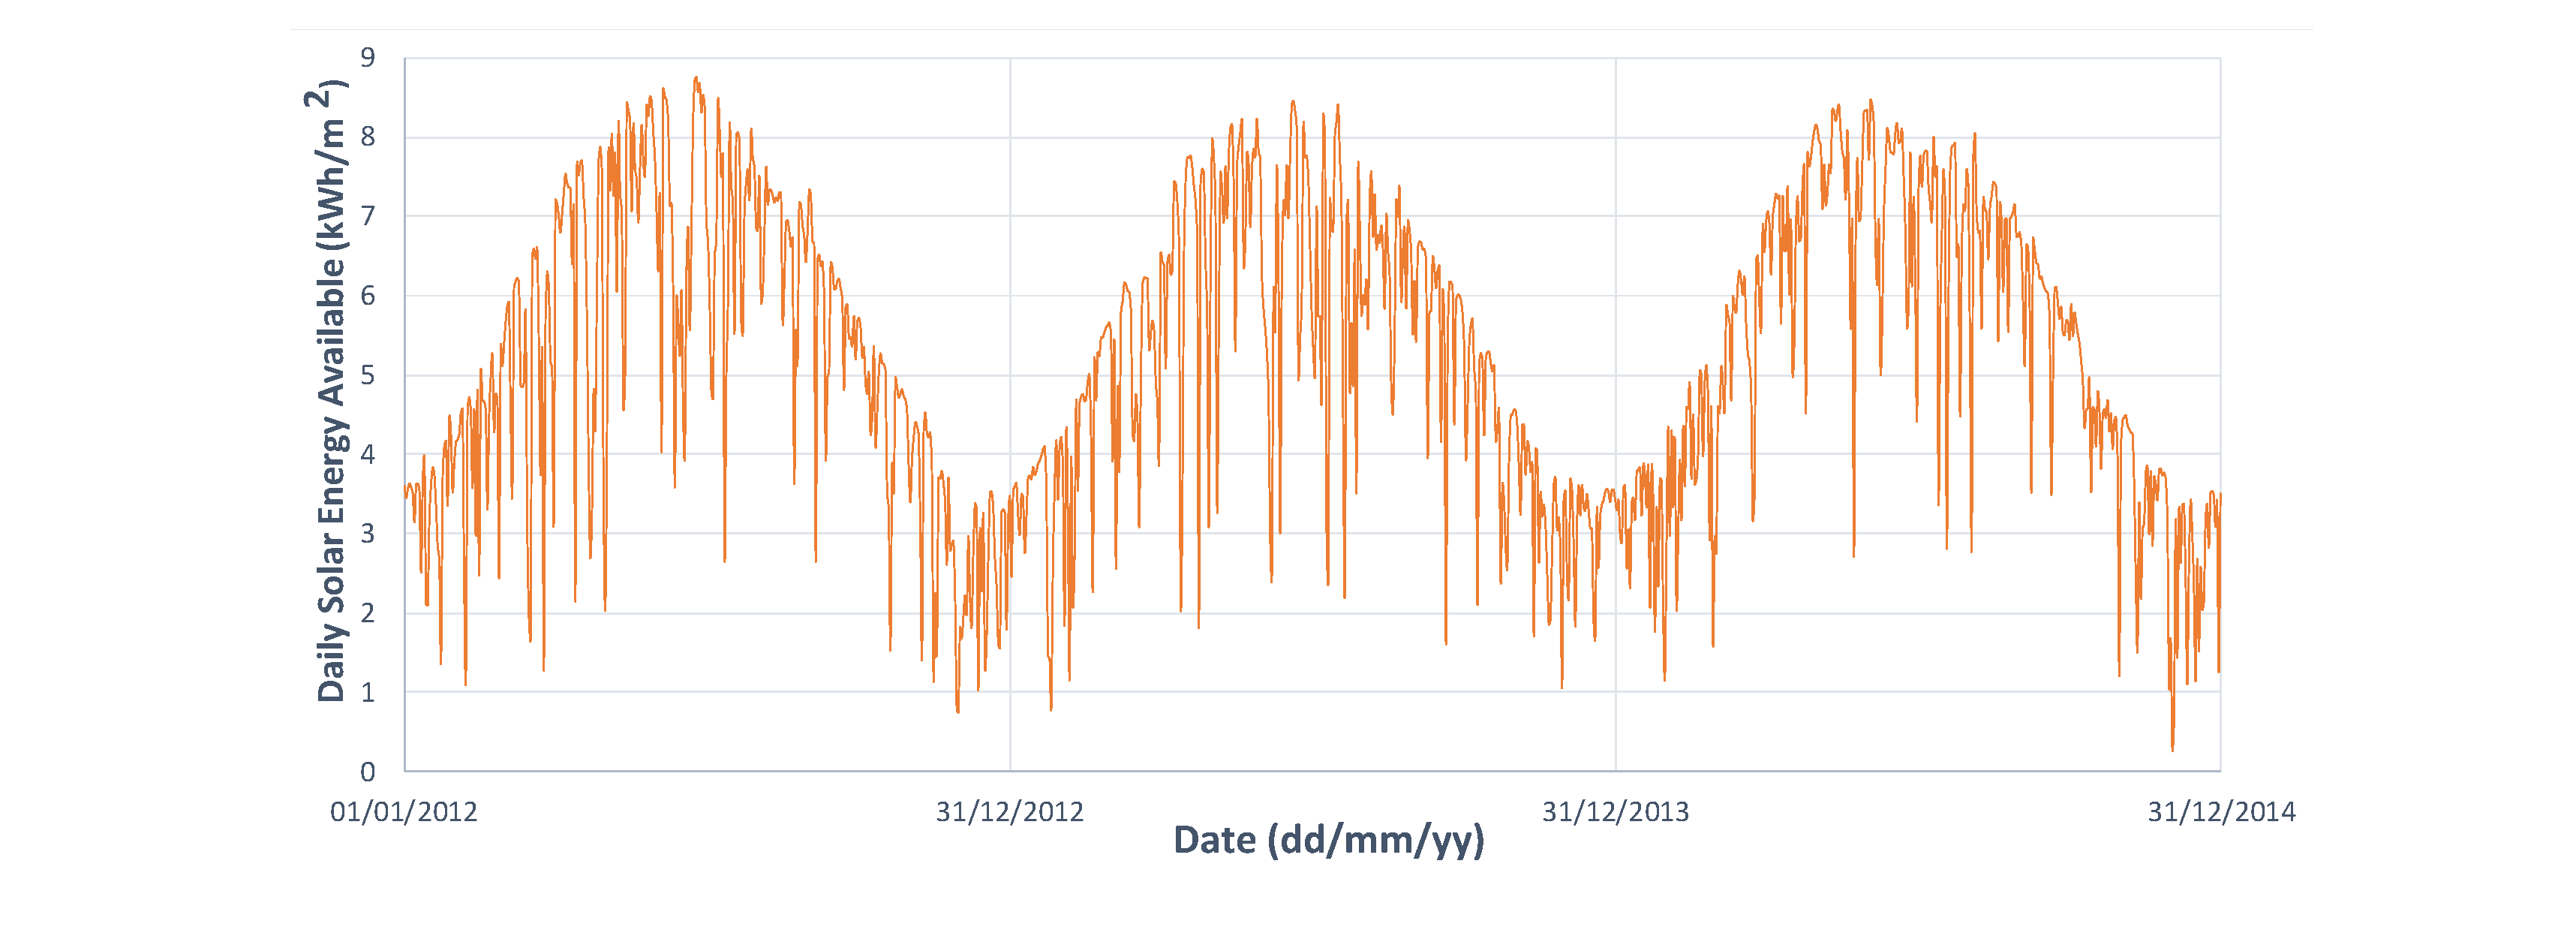
\includegraphics[width=14cm]{ch2_review/figures/solar_calendar}
    \caption{Daily global horizontal solar energy available in Los Angeles 2012-2014~\cite{nreldata}.}
    \label{Figure:solar_calendar}
\end{figure}

\begin{figure}[!htb]
    \centering
    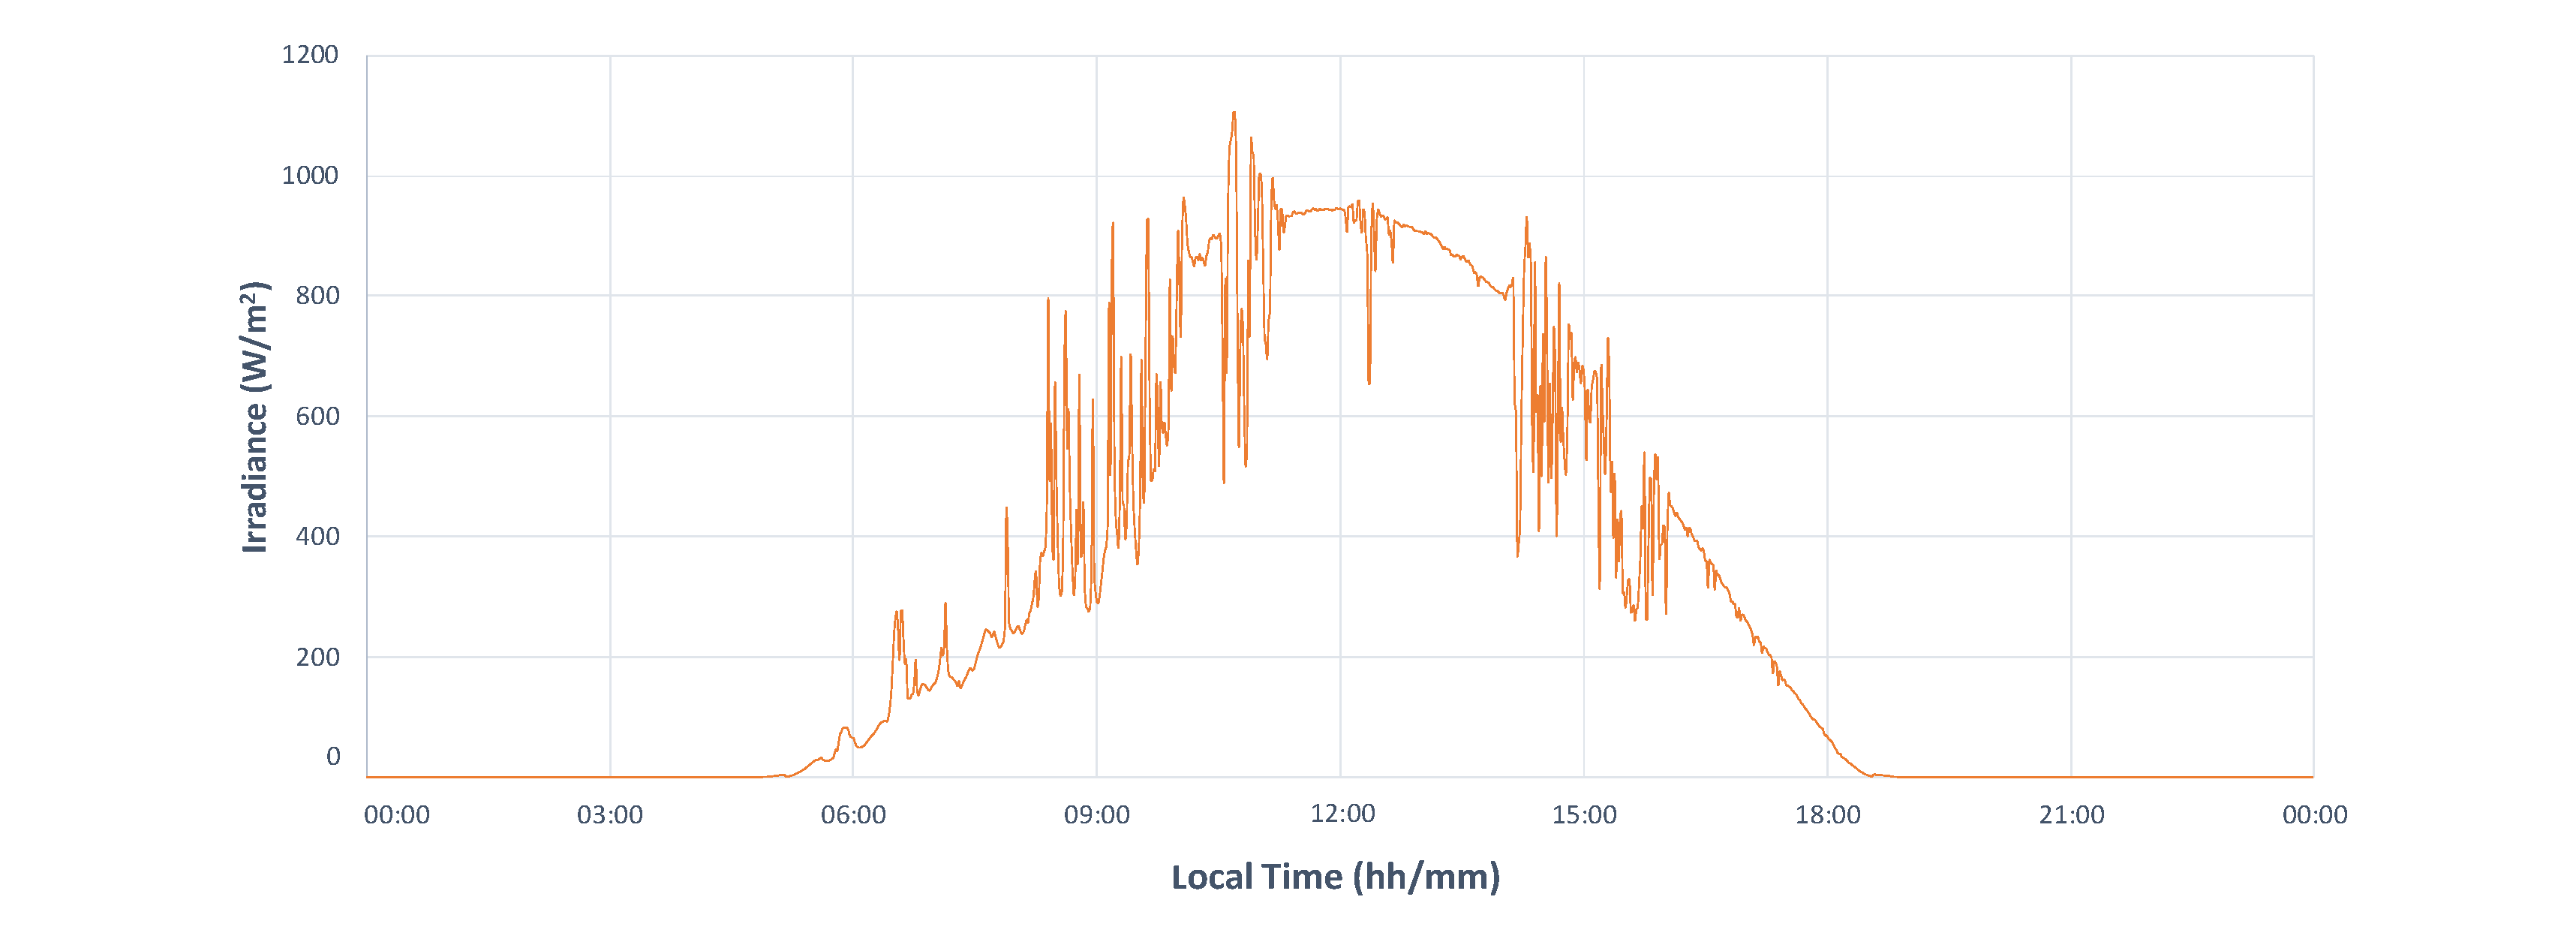
\includegraphics[width=14cm]{ch2_review/figures/solar_plots}
    \caption{One-day dynamics of global horizontal solar irradiance in Los Angeles 29 April 2016~\cite{lmu}.}
    \label{Figure:solar_plots}
\end{figure}

In order to make full use of solar energy, substantial efforts have been made to develop and improve energy harvesting sensor nodes with solar panels~\cite{raghunathan2005design, seah2009wireless}. Generally, solar energy harvesting approaches adopt large energy storage, e.g. a rechargeable battery, to smooth out the daily and annual variations. Examples of solar-powered sensor nodes are presented in~\cite{raghunathan2005design, corke2007long, kansal2007power}, and a comprehensive review on solar-powered sensor nodes is published in~\cite{sudevalayam2011energy}. 

\subsection{Radio Frequency Energy Harvesting}

Radio Frequency (RF) energy exists in time-varying electromagnetic fields, which widely spread in our environment now due to the propagation of wireless networks, such as Wi-Fi and cellular phone signals~\cite{parks2013wireless}. When radio waves pass through an antenna, due to electromagnetic induction, AC voltage is generated. This AC voltage can be rectified and regulated to DC power for sensor nodes. The received RF power is reciprocal to the square of distance from the source to the destination. The maximum conversion efficiency from RF waves to DC power is typically 50-75\% given a transmission distance of 100 metres~\cite{shaikh2016energy}.
% received power?

Due to the widespread deployment of telecommunication networks, RF energy harvesting becomes available in a wide range of locations, both outdoors and indoors. Compared to light energy harvesting, RF harvesting shows its strength in indoor applications as there is often low or no light intensity inside buildings. 

A basic and common example of RF harvesting is RF Identification (RFID). In a passive RFID application, an RFID reader transmits RF signals to an RFID tag for asking its tag information. The tag absorbs the signals and energy through its antenna, and then responds the reader with its information. Up to now, Wireless Identification and Sensing Platform (WISP)~\cite{sample2008design, naderiparizi2015wispcam} is presented to show the possibility of the integration of RF energy harvesting in IoT applications.

\subsection{Flow Energy Harvesting}

Flow-based energy harvesting utilises turbines and rotors to collect the kinetic energy in air flow or liquid flow. Air flow is converted by wind turbines and liquid flow is converted by hydrogenerators. Wind turbines and hydrogenerators are normally in different mechanical structures (shapes), but the fundamental principles of them are the same.

% Wind turbines are another kind of mature energy harvesters besides PV techniques. 
Wind turbines are manufactured in a wide spectrum in terms of dimensions, from a large-scale wind farm (arrays of large turbines) to a portable micro wind turbine. Micro wind turbines are suitable for battery charging and powering autonomous electronic devices. 

\begin{figure}[!htb]
    \centering
    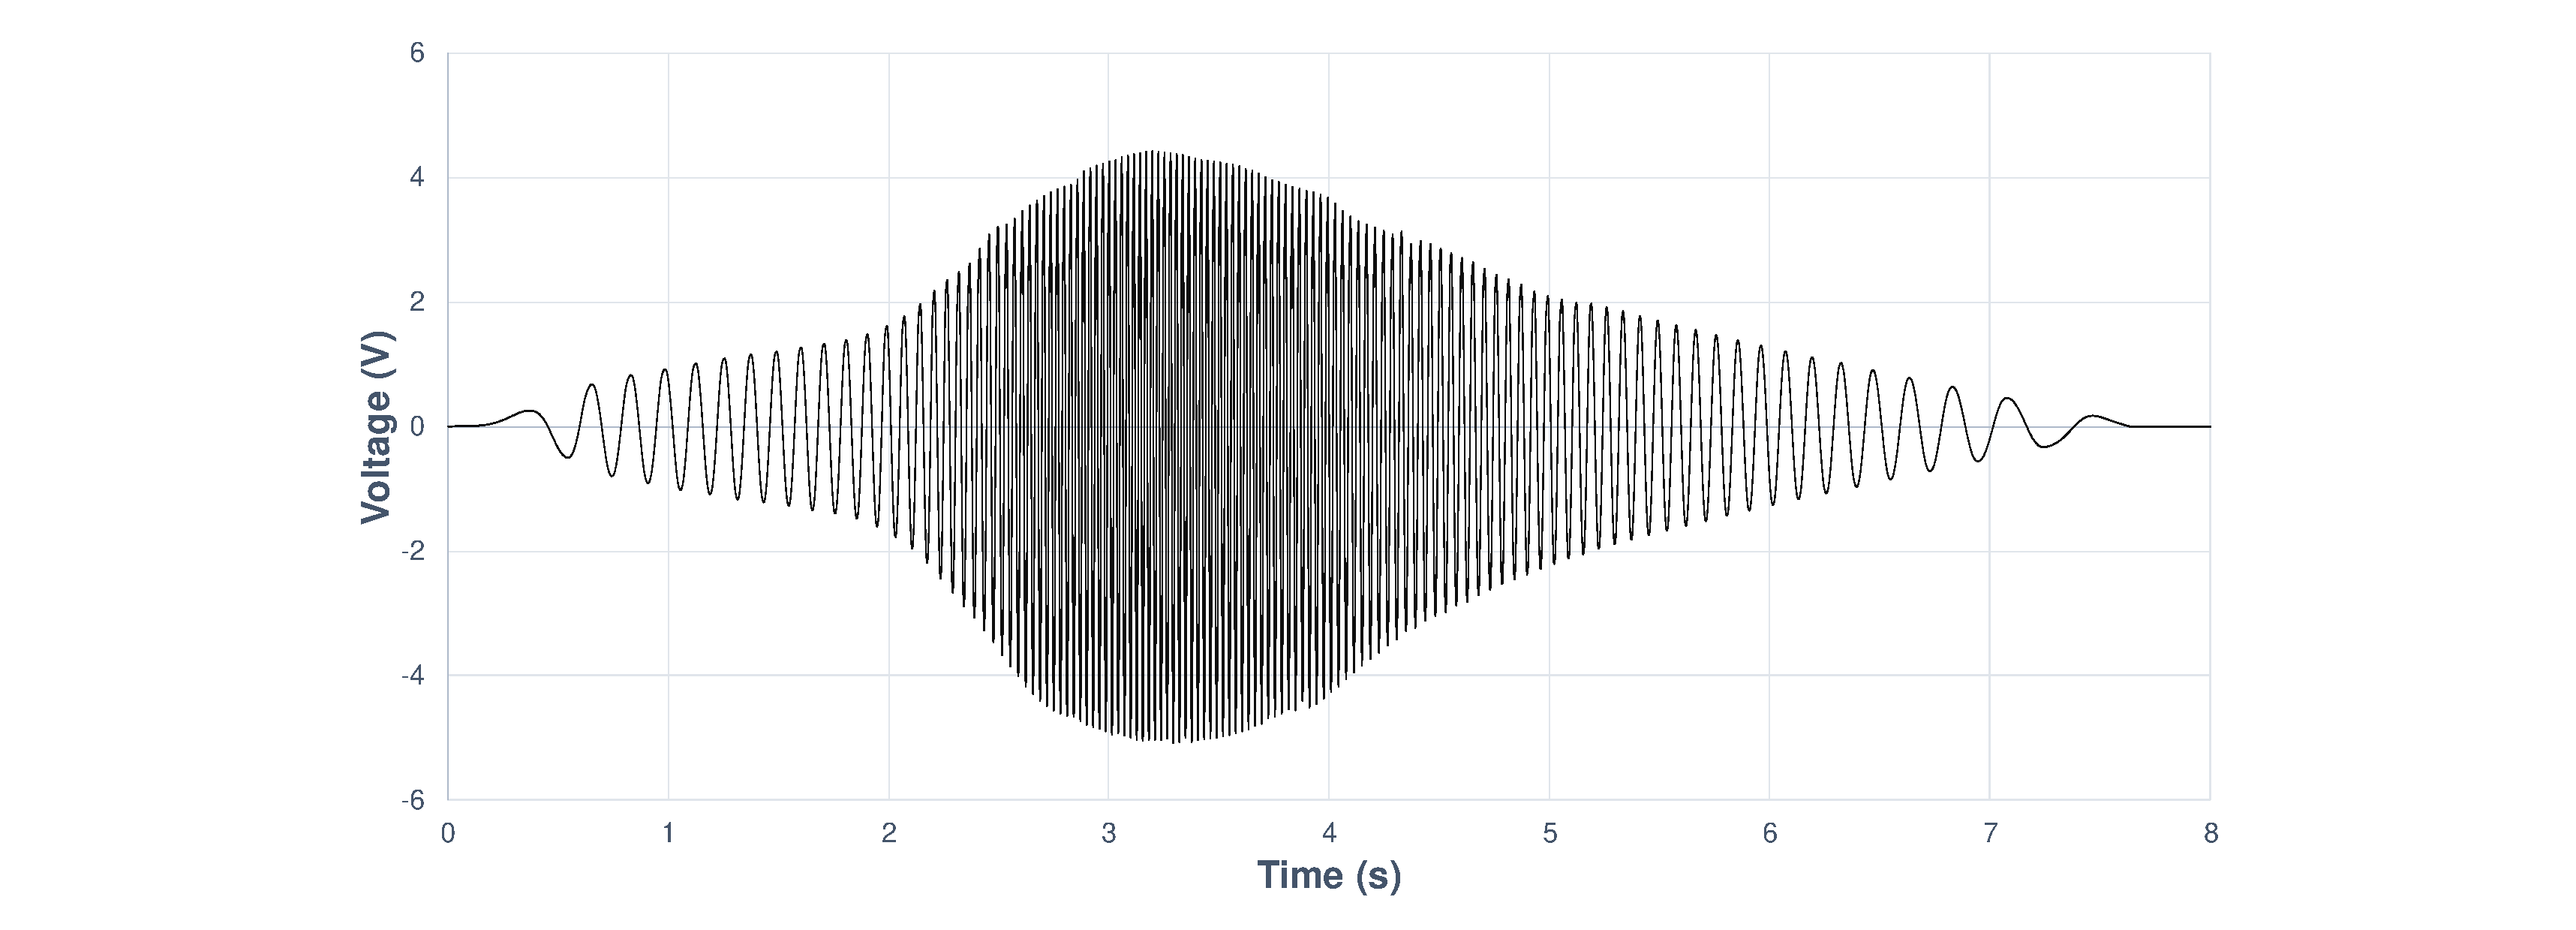
\includegraphics[width=14cm]{ch2_review/figures/micro_wind_turbine}
    \caption{Dynamics of a micro wind harvester (reproduced from~\cite{balsamo2016graceful}).}
    \label{Figure:micro_wind_turbine}
\end{figure}

A raw voltage output trace of a micro wind turbine given a blast of wind is presented in~\fref{Figure:micro_wind_turbine}. Given a constant blow, a wind turbine should produce a sinusoidal voltage signal. Its voltage output vibrates from the positive domain to the negative domain with time, so a rectifier is normally required in order to utilise this AC power for DC load.

Similar to solar energy, wind energy is uncontrollable but partially predictable. Sharma \textit{et al.}~\cite{sharma2010cloudy} introduce a system that achieves available wind energy predictions based on downloaded weather forecast information within recent 3 days. Also, Cammarano \textit{et al.}~\cite{cammarano2012pro} present a wind and solar energy predicting method which dynamically adjusts its time horizon of prediction in order to achieve higher accuracy than its prior methods. 

Hydrogenerators harness the energy in moving liquids, such as water or a mix of different liquids. Traditionally, hydrogenerators are used for generating large-scale electricity from rivers and streams. However, since the possible underwater applications in IoT, hydrogenerators can be a suitable alternative for powering sensor nodes. For example, Morais \textit{et al.}~\cite{morais2008sun} incorporate a small-sized hydrogenerator as a part of energy harvesting supply for sensor nodes. 

%\fref{Figure:piezo} plots the theoretical rectified power output of a piezoelectric harvester designed in a portable size, as a function of the load resistance $\mathbf{R}$ and the squared coupling coefficient $\mathbf{k^2}$ give a constant external force, where $\mathbf{k^2}$ means the energy conversion efficiency of a piezoelectric material. As observed from \fref{Figure:piezo}, there are one or two optimal loads with the variation of $\mathbf{k^2}$, and with the increase of $\mathbf{k^2}$, the power output approaches a maximum value \cite{shu2006analysis}.

% Mechanical
% \subsection{Mechanical Energy Harvesting}

% Piezoelectricity is the electric effect resulted from the mechanical pressure on certain solid materials, such as lead zirconate titanate (PZT) and polyvinylidene fluoride (PVDF). It is usually used for harvesting vibration and motion energy generated by machines and human walking~\cite{shu2006analysis}. 

% The exemplary power production under certain harvesting conditions is listed in \tref{Table:sources}.

% \begin{table}[!htb]
%     \centering
%     \begin{tabular}{|c|c|c|}
%     \toprule
%     \textbf{Harvester} & \textbf{Energy Source} & \textbf{Harvested Power}\\
%     \midrule
%     Piezoelectric & Footfalls & 1.3mW \cite{shenck2001energy}\\
%     Thermoelectric & Human body heat & 2mW\cite{leonov2013thermoelectric}\\
%     RF & Radio signal & 15.8$\mu$W \cite{parks2013wireless}\\
%     \bottomrule
%     \end{tabular}
%     \caption{Power outputs of various energy harvesters}
%     \label{Table:sources}
% \end{table}

% Thermal Energy
% \subsection{Thermal Energy Harvesting}

% Thermoelectric generators can produce electricity from a temperature difference utilizing the Seebeck effect. This thermal difference can come from human body, industrial devices, geological effects, etc~\cite{beeby2010energy}. 

\section{Energy Storage for Sensor Nodes} \label{Section:ES}
% if this is the tile, should I mention primary batteries?

Energy harvesting supply is variable and intermittent over time, causing disparity between power supply and power consumption. In order to deliver stable power output from a varying source, a critical component in an energy harvesting power unit is energy storage, which buffers the harvested energy and powers the load when needed. Besides its ability to buffer energy and its effect on overall efficiency, energy storage has a dominant effect on the size, cost, and lifetime of sensor nodes~\cite{akhtar2015energy}. Therefore, how to design energy storage is a critical concern in deploying energy harvesting sensor nodes. 

Technologies of energy storage used in sensor nodes are generally divided into two categories: rechargeable batteries and capacitors, which are different from each other in terms of energy density, power density, lifetime, discharging features, leakage, etc. In general, batteries have higher energy density (containing more energy with the same volume/weight), lower leakage, and a more stable discharging curve (a stable voltage output while discharging), while capacitors have higher power density (higher limits for charging/discharging current), and longer lifetime in terms of charge-discharge cycles~\cite{raghunathan2005design, akhtar2015energy}. The choice of these two forms of energy storage depends on application requirements. These two technologies and their implementations will be briefly reviewed in the following subsections.

\subsection{Rechargeable Batteries}

Batteries are more energy-dense than capacitors and manifest a stable voltage output when discharging. Rechargeable batteries have been widely adopted in mobile devices. Rechargeable batteries are generally made in the following techniques: Sealed Lead Acid (SLA), Nickel Cadmium (NiCd), Nickel Metal Hydride (NiMH), Lithium Ion (Li-ion), and Lithium ion Polymer (Li-Po). Due to the similar techniques and features of Li-ion and Li-Po batteries, Li-ion will be used to represent Li-ion and Li-Po batteries in this subsection. SLA and NiCd batteries are less likely to be implemented in energy harvesting sensor nodes~\cite{raghunathan2005design, akhtar2015energy}. SLA batteries suffer from low energy density and are normally bulky and heavy, which is unfavorable for sensor nodes. NiCd batteries involve memory effect, i.e. decrease of energy capacity after repeated partially discharging and recharging, which is a common situation in energy harvesting implementations. 

% NiMH and Li-ion, their advantages and disadvantages. Comparison with a table. 
 Compared to SLA and NiCd batteries, NiMH and Li-ion batteries show a strength in energy density in both weight and volume, and hence, are more suitable for energy harvesting applications~\cite{raghunathan2005design, taneja2008design, akhtar2015energy, prauzek2018energy}. A comparison of two commercial NiMH and Li-ion batteries is listed in~\tref{Table:nimhliion} with a variety of perspectives and features. Li-ion batteries are typical lighter than NiMH batteries, with weight energy density 2-3x and volume energy density 1-2x to NiMH batteries. Also, Li-ion batteries significantly outperform NiNH batteries in terms of charging efficiency and self-discharge rate. However, Li-ion batteries are normally more expensive than NiMH batteries, and require more complicated pulse charging circuits~\cite{raghunathan2005design}. NiMH batteries also provide a relatively constant voltage supply during discharging~\cite{kansal2007power}. 

\begin{table}[!htb]
    \centering
    \begin{tabular}{ccc}
    \toprule
    & NiMH (Panasonic BK150AA) & Li-ion (EEMB LIR14500) \\
    \midrule
    Nominal voltage & 1.2 V & 3.7 V \\
    Charge capacity & 1500 mAh & 750 mAh \\
    Energy capacity & 1.80 Wh & 2.775 Wh \\
    Weight & 26 g & 20 g \\
    Dimensions & \diameter14.5mm $\times$ 50.5mm & \diameter14.1mm $\times$ 48.5mm \\
    Weight energy density & 69 Wh/Kg & 139 Wh/Kg \\
    Volume energy density & 216 Wh/L & 366 Wh/L \\
    Operating temperature & -20$^\circ$C to 65$^\circ$C & -20$^\circ$C to 60$^\circ$C \\
    Charging cycles & \multirow{2}{*}{$>$500} & \multirow{2}{*}{$>$300} \\
    (until 80\% capacity) & & \\
    Reference price & $\pounds$2.91 & $\pounds$3.25 \\
    Charging efficiency~\cite{prauzek2018energy} & 66\% & 99.9\% \\
    Self-discharge~\cite{prauzek2018energy} & 30\% per month & 10\% per month \\
    Charging Method~\cite{prauzek2018energy} & Trickle & Pulse \\
    \bottomrule
    \end{tabular}
    \caption{Comparison between commercial NiMH and Li-ion rechargeable batteries.}
    \label{Table:nimhliion}
\end{table}

NiMH and Li-ion batteries have been widely implemented in energy harvesting sensor nodes. Heliomote~\cite{raghunathan2005design} uses two NiMH batteries in series to match the charging voltage (2.2-2.8V) with the MPP of the solar panel. HydroSolar~\cite{taneja2008design} also adopts two NiMH batteries to avoid the Li-ion charging hardware. Jiang \textit{et al.}~\cite{jiang2005perpetual} design a hybrid storage system including a lithium based rechargeable battery as the secondary buffer, due to its high efficiency and charge density.

Despite the high energy density and stable discharging voltage, batteries still show a typical drawback at short lifetime (less than 5 years~\cite{simjee2008efficient}), which involves manual replacement of batteries or devices after the battery lifetime expires. Also, batteries raise environmental concerns due to the heavy metals and toxic chemicals within. If not properly charged, Li-ion batteries can cause safety issues, i.e. explosion and fire, which are problematic when deployed in distant and wild places. In addition, rechargeable batteries are susceptible to temperature. Most batteries only exhibit their rated characteristics around 20$^\circ$C, and lose their efficiency and capacity when operating at extreme temperatures (around their rated limits)~\cite{prauzek2018energy}. 

 % mention the two new papers from Neal Jackson?

\subsection{Capacitors}
% leakage and lifetime of supercapacitors???

Due to the lifetime limits and pollution issues of batteries, capacitors, typically supercapacitors, are considered as an alternative to replace rechargeable batteries as energy storage. Supercapacitor (also known as ultracapacitors or electrostatic double-layer capacitors) are capacitors with higher energy density than electrolytic capacitors. Unlike conventional capacitors, where charges are stored and separated by solid dielectric, supercapacitors maintain charges based on double-layer or pseudo-capacitive charging phenomena~\cite{bueno2019nanoscale}. Supercapacitors are still much less energy-dense than batteries, but act as a transition from capacitors to batteries. 

Compared to rechargeable batteries, supercapacitors exhibit strengths in a large number of charge/discharge cycles, long lifetime (20 years), high charge/discharge efficiency (98\%). The self-discharge rate of supercapacitors is higher than batteries, with 5.9-11\% of maximum capacity per day~\cite{libich2018supercapacitors, renner2009lifetime}, but this leakage is insignificant compared to the small capacity and the total energy gained per day. The main constraint of supercapacitors is still the low energy density, which results in large storage dimensions if the aim were to achieve a comparable capacity with batteries. In order to maintain the same form factors of sensor nodes, designers have to adapt system architecture to a small storage (compared to batteries).

Prometheus~\cite{jiang2005perpetual} introduces supercapacitors into energy storage for sensor nodes whereby two 22F supercapacitors are used in combine with a Li-Po battery. AmbiMax~\cite{park2006ambimax} also proposes a hybrid storage design similar to Prometheus, but with two more 10F supercapacitors for wind energy harvesters. To achieve longer lifetime than battery-based sensor nodes, Everlast~\cite{simjee2006everlast} demonstrates the feasibility of replacing batteries with supercapacitors in energy harvesting sensor nodes, designing a power system that adopts a 100F supercapacitor as the only energy reservoir. 

However, farad-level supercapacitors occupy a significant part of device volume. The advent of energy-driven computing~\cite{merrett2017energy} introduces the application and design scenario where execution happens only if there is energy available. Within this scenario, energy storage using millifarad-level supercapacitors are investigated in energy harvesting sensing applications~\cite{naderiparizi2015wispcam, gomez2016dynamic}. Furthermore, intermittent computing, which will be illustrated in the next section, enables computation given intermittent power, making progress with electrolytic capacitors or even without dedicated storage (only microfarad-level parasitic capacitance).

\subsection{Discussion}

To summarise, due to the requirements on lifetime, environmental-friendliness, and form factors in energy harvesting sensor nodes, the energy storage designs have transformed from batteries to supercapacitors, and eventually eliminated the need for dedicated storage. 

Batteries have been the preferable choice for buffering harvested energy and powering sensor nodes because they make sensor nodes easy to program and operate reliably until the battery lifetime expires. However, the environmental issues and short lifetime of batteries limit the deployment of ubiquitous sensors. Supercapacitors avoid the problems of batteries and have been used to replace batteries, but the low energy density of supercapacitors also makes sensor nodes bulky and heavy in order to achieve sufficient capacity for uninterrupted operations. Recent development of intermittent computing enables forward execution over power outages and encourages storage-less designs in energy harvesting sensor nodes.

Although the minimum need for storage capacity to operate sensor nodes decreases with the evolution of computing techniques, decreased storage does limit the flexibility of energy usage. A storage-less system has to consume the incoming power immediately, otherwise the energy is wasted. This fact consequently restricts the application scenarios of storage-less systems to energy-driven applications, where execution needs to run only when there is available energy sources to harvest. However, energy-driven applications do not cover all the demands in IoT, so simply reducing the storage need is not always desirable. A wider spectrum of storage designs should be explored to suit and optimise for different application scenarios.

% \begin{center}
%     \begin{tabular}{|c|c|c|c|} 
%     \hline
%     Capacitance ($\mu F$) & Aluminum(10V)[1] & Aluminum(10V)[2]  & Tantalum(10V)[3]\\ [1ex] 
%     \hline\hline
%     22 & 5$\times$11 & 5$\times$11 & 5.5$\times$10.5\\ 
%     \hline
%     47 & 5$\times$11 & 5$\times$11 & 6.5$\times$11.5\\
%     \hline
%     100 & 5$\times$11 & 5$\times$11 & 8.5$\times$14\\
%     \hline
%     220 & 6.3$\times$11 & 6.3$\times$11 & 10$\times$17\\
%     \hline
%     330 & 8$\times$11.5 & 8$\times$11.5 & 10$\times$18.5\\
%     \hline
%     470 & 8$\times$11.5 & 8$\times$11.5 & N/A\\
%     \hline
%     1000 & 10$\times$12.5 & 10$\times$16 & N/A\\
%     \hline
%     \end{tabular}
% \end{center}

\section{Energy-Neutral Computing} \label{Section:EN}

Energy-neutral (EN) computing aims to operate sensor nodes with at least a certain performance level over a period of time. Energy-neutrality can be described as the following equation:

\begin{equation} \label{eq:energyneutral}
    E_{min} \leq E_{t_0} + \int_{t_0}^{t_0+\Delta t} [P_h(t) - P_c(t)] dt \leq E_{max}
\end{equation} 

where $P_h(t)$ and $P_c(t)$ are the harvested and consumed power at time $t$, $t_0$ is the time when EN computing is meant to start, $\Delta t$ is the length of period during which EN conditions are achieved, $E_{t_0}$ is the initial available energy in energy storage at time $t_0$, $E_{min}$ is the minimum amount of stored energy below which the system cannot sustain (typically due to insufficient supply voltage), and $E_{max}$ is the maximum capacity of energy storage beyond which the harvested energy is wasted. $P_c(t)$ includes the power consumption of the whole system, such as the MCU, peripherals, power conversion circuit, and the power leakage of energy storage. $P_h(t)$ is the harvested power after conversion. 

EN devices are typically powered by solar cells~\cite{escolar2014energy}, and $\Delta t$ is typically 24 hours or one year to suit the period of the solar energy source. In order to achieve energy neutrality over such a long term, sufficient amount of energy storage, typically in the form of rechargeable batteries, is required to smooth out the large temporal variations of harvested power. The capacity of the energy storage is determined by how long the system tries to maintain a stable performance as larger energy storage tolerates more energy differences. In general, the length of $\Delta t$ and the difference between $P_h$ and $P_c$ determine how much storage is required, and on the other hand, the capacity of energy storage limits how long $\Delta t$ can be.

In order to ensure that the system works uninterruptedly by managing the stored energy (the middle term in Equation~\ref{eq:energyneutral}) between $E_{min}$ and $E_{max}$, EN computing dynamically adapts system performance and power consumption over the period $\Delta t$. Typical adapting techniques include adjusting workload duty cycles and participation in network activity~\cite{merrett2017energy}.

% In the following part of this section, most of the mentioned power management methods are based on solar energy harvesting.

Kansal \textit{et al.}~\cite{kansal2007power} illustrate a preliminary power management algorithm by which the incoming energy is estimated by an Exponentially Weighted Moving Average (EWMA) of the past recorded slots of harvested energy, and the system tries to exploit the harvested energy by scaling its duty cycles. Vigorito \textit{et al.}~\cite{vigorito2007adaptive} introduce a Linear-Quadratic Tracking (LQT) approach to scale duty cycles based on the current battery level, and as evaluated in its datasets, mean duty cycle is improved by 6-32\% and duty-cycle variation is reduced by 6-69\% compared to~\cite{kansal2007power}, which means the system works with a more a stable performance. In~\cite{le2012power}, a Proportional-Integral-Derivative (PID) controller is used for monitoring and stabilizing the voltage of a supercapacitor-based energy storage, and hence, the storage level of this system. While these approaches achieve satisfactory energy neutrality for the magnitude of hours, they all show a latency when responding to the harvested power, and high variance of duty cycles when adapting to a new power trace. Additionally, approaches in~\cite{vigorito2007adaptive} and~\cite{kansal2007power} rely on an accurate estimating algorithm to detect the remaining battery energy, which is vulnerable to deployed time and temperature. 

In~\cite{piorno2009prediction}, a prediction algorithm for solar energy named Weather-Conditioned Moving Average (WCMA) is presented, in which both the current and the past weather data are taken into account to achieve higher accuracy than EWMA methods. It is reported by the authors that the average prediction error is improved from 28.6\% in EWMA to 9.8\% in WCMA over a test duration of 45 days, but it is unclear in the article that how to harness this prediction to improve the system performance. Similarly, weather forecast is adopted in~\cite{sharma2010cloudy}, by which the authors build a model to approximate the available solar and wind energy. Although these two methods based on weather data provide high prediction accuracy, the network overheads for receiving these data are not presented, and how to fully utilise this daily prediction is still a problem.

Different from the aforementioned daily EN operations, a long-term annual power management based on duty-cycling is presented in~\cite{buchli2014dynamic} to achieve annual energy neutrality. The authors use an adjustment factor, which is dynamically calculated from the historical windows, to modify the design-time energy prediction model to a more realistic model, and determine its performance level accordingly. However, this algorithm is only tested in simulation instead of practical experiments. Moreover, for such a long-term EN operation, a large battery is required, but the battery deterioration is ignored in their analysis.

In~\cite{caruso2018dynamic}, a task scheduling algorithm for optimising the performance of an energy harvesting system (typically based on PV harvesters) is exhibited. Given a predicted power trace, storage bounds, energy consumption of tasks and quality of tasks, the proposed scheduling algorithm is proved to be able to find the optimal scheduling in a pseudo-polynomial time which leads to the maximum sensing quality. While this algorithm provides an ideal solution for power management, it requires that the energy source should be predictable with high accuracy, and the energy cost and quality of each task should be defined at design time. The first requirement almost constrains this algorithm within the cooperation of solar energy. The second requirement is hard to achieve since a) in practice the energy consumption of tasks may change due to temperature and dynamic data amount~\cite{walker2016thermally} and b) the energy cost of a system includes many elements other than the energy consumption of computing tasks.

EN computing efficiently utilises energy and maintains system performance, ensure reliability and periodic task execution despite variable harvesting power input. However, in almost all energy neutral approaches reviewed above, a large energy storage, i.e. a rechargeable battery, is in need in order to buffer temporal energy variations. The usage of batteries poses sustainability challenges due to the limited lifetime and pollution issues. Recent research develops intermittent computing and power-neutral computing, which minimise the need for energy storage. The next two sections (Section \ref{Section:IC} and Section \ref{Section:PN}) review the methodologies of these two research topics. 

\section{Intermittent Computing} \label{Section:IC}

Energy harvesting provides an autonomous power supply for wireless sensor nodes as an alternative of battery power. However, with small storage, energy harvesting systems inevitably suffer from frequent power outages, which affect forward execution of programs. Intermittent computing (IC, also known as transient computing) aims to maintain forward execution and computation correctness through power failures~\cite{ransford2012mementos}. Intermittent execution spans its execution and intermittently computes over power outages, while conventional execution restarts after power interrupts. A typical characteristic of an IC system is that it starts executing whenever there is power available and suspends during power outages; after power recovery, it can continue its prior task correctly instead of restarting from the beginning of a program. 

Due to different design considerations, the methodologies in IC varies in a wide spectrum~\cite{sliper2018enabling}. These methodologies include saving snapshots of system state to non-volatile memory (NVM), breaking down execution into small tasks, hardware circuits for suspend and restore operations, etc. The existing IC approaches can be classified into four types: checkpointing, reactive IC, task-based IC, and non-volatile processors (NVP). The following part of this section explains the each methodology one by one, as well as their works and current research progress.

\subsection{Checkpointing IC}

Checkpointing IC inserts checkpoints into code at compile time. When a checkpoint is called, the system checks the current available energy amount. If this amount is less than a predefined threshold, which indicates the available energy may not be enough to sustain execution, a snapshot saving function is called at this checkpoint. To save a snapshot of the system computing state, the system copy current stacks and heaps, local and global variables, general registers, the stack pointer, and the program counter, into the NVM. A checkpointing system continuously operates until it encounters power outages, where the supply voltage is less than the minimum operating voltage of the systems. After the supply voltage recovers, the system restore its state from the last checkpoint, and hence, continue its execution from that checkpoint. 
% a figure here explaining the control flowing of checkpointing?

Mementos~\cite{ransford2012mementos} first provides a checkpointing solution in which checkpoints are planned at compile time. Mementos includes three strategies of placing checkpoints, which are placing at every loop, placing at every function call, and an auxiliary timer delay to determine the minimum cycle between two adjacent checkpoints. Additionally, programmers can also insert or delete checkpoints manually as a custom option. Two NVM blocks are used and snapshots are saved to the two blocks alternately, so there is always at least one available and complete snapshot even if the energy is depleted during saving a new snapshot. One significant shortcoming of Mementos is the instrumenting strategy: with the different sizes of loops and functions, the granularity of checkpoints can be either too small, which introduces high run-time overheads, or too large, which leads to non-termination where the execution can never get to the next checkpoint. It is a concern in Mementos that how to set the voltage threshold which triggers saving snapshot. Setting this too high leads to redundant snapshots, while setting this too low leads to the failure of saving snapshots and cannot guarantee forward progress.

HarvOS~\cite{bhatti2017harvos} is proposed to improve the strategies of inserting checkpoints in Mementos. HarvOS analyses the control-flow graph of a program and splits it into sub-graphs with a checkpoint inserted for each sub-graph. To reduce the number of checkpoints compared to Mementos, the size of sub-graphs is set close to the worst-case number of useful cycles the MCU can execute until the next checkpoint. To reduce the size of snapshots, the RAM usage in each sub-graph is analysed and the checkpoint is placed at the point with the least RAM usage. HarvOS claims to reduce 68\% checkpoints on average compared to Mementos.

Chinchilla~\cite{maeng2018adaptive} proposes a checkpointing tool which automatically overprovisions checkpoints at compile time and adaptively eliminates unnecessary checkpoints at run time. Compared to Mementos and HarvOS, Chinchilla relieves the programming efforts on manually inserting checkpoints while still achieves an efficient number of checkpoints at run time.

An advantage of the checkpointing method is the size of a specific snapshot can be estimated from the program execution flow to find a smaller snapshot~\cite{bhatti2017harvos}. However, there are still two significant challenges remaining unsolved in checkpointing methods: idempotency violation and non-termination. 

An execution is idempotent if it can be repeated while maintaining the same result~\cite{lucia2015simpler}. Non-idempotent actions include I/O operations and NVM writes, which are fairly common in IC applications. Repeating non-idempotent actions can leads to undesired results, so these non-idempotent actions should be executed only once. Checkpointing systems repeat executing the code between two adjacent checkpoints, and hence, cause non-idempotency. Current compile-time checkpointing methods as listed above are not able to ensure idempotency. 

Non-termination in checkpointing systems exhibits when the energy consumption of execution between two checkpoints is too much that the system energy buffer and harvested supply cannot sustain. Non-termination typically happens when the instrumentation strategy of checkpoints ignores the size of the energy buffer, as in Mementos. HarvOS and Chinchilla manage to mitigate non-termination, but they cannot eliminate this problem as they cannot dynamically insert checkpoints at run time according to varying environmental sources. 
% Main drawbacks: idempotency, non-termination/deadlock.

\subsection{Reactive IC} \label{Section:reactiveic}

Instead of instrumenting checkpoints at compile time, reactive IC does not set predefined checkpoints but save snapshots at run time when the supply voltage is detected to be lower than a threshold that indicates an imminent power failure. Therefore, the snapshot saving operations is only invoked when there is an indication of an imminent power outage, i.e. a low supply voltage. Also, after saving a snapshot, a reactive IC system suspends its execution and enter a low-power mode, rather than continues execution until a power outage as checkpointing systems do. When the voltage supply recovers above a restore threshold, the system either restores the last snapshot if the system reboots, or just continues execution if the system comes back from the low-power mode.

Hibernus~\cite{balsamo2015hibernus} saves only one snapshot before a power interruption and then enter the sleep mode. Two fixed voltage thresholds, $V_H$ and $V_R$, are predefined for hibernation (save a snapshot and sleep) and restoring a snapshot. An on-chip voltage comparator and an on-chip voltage reference generator are used for monitoring the supply voltage and triggering hibernation when the supply voltage drops to $V_H$ or restoration when the supply voltage recovers to $V_R$. A voltage trace is shown in~\fref{Figure:hibernus} to explain Hibernus behaviours, and this trace is representative for a reactive IC system behaviours. To adapt thresholds to variable energy sources, Hibernus++~\cite{balsamo2016hibernus++} implements dynamic self-calibration for suspend and restore thresholds by executing a hibernation test. By using adaptive thresholds instead of fixed thresholds as in Hibernus, Hibernus++ makes itself compatible with a variety of energy sources. Compared to Hibernus, Hibernus++ improves application execution time by reducing the overheads of suspend and restore operations.

\begin{figure}[!htb]
    \centering
    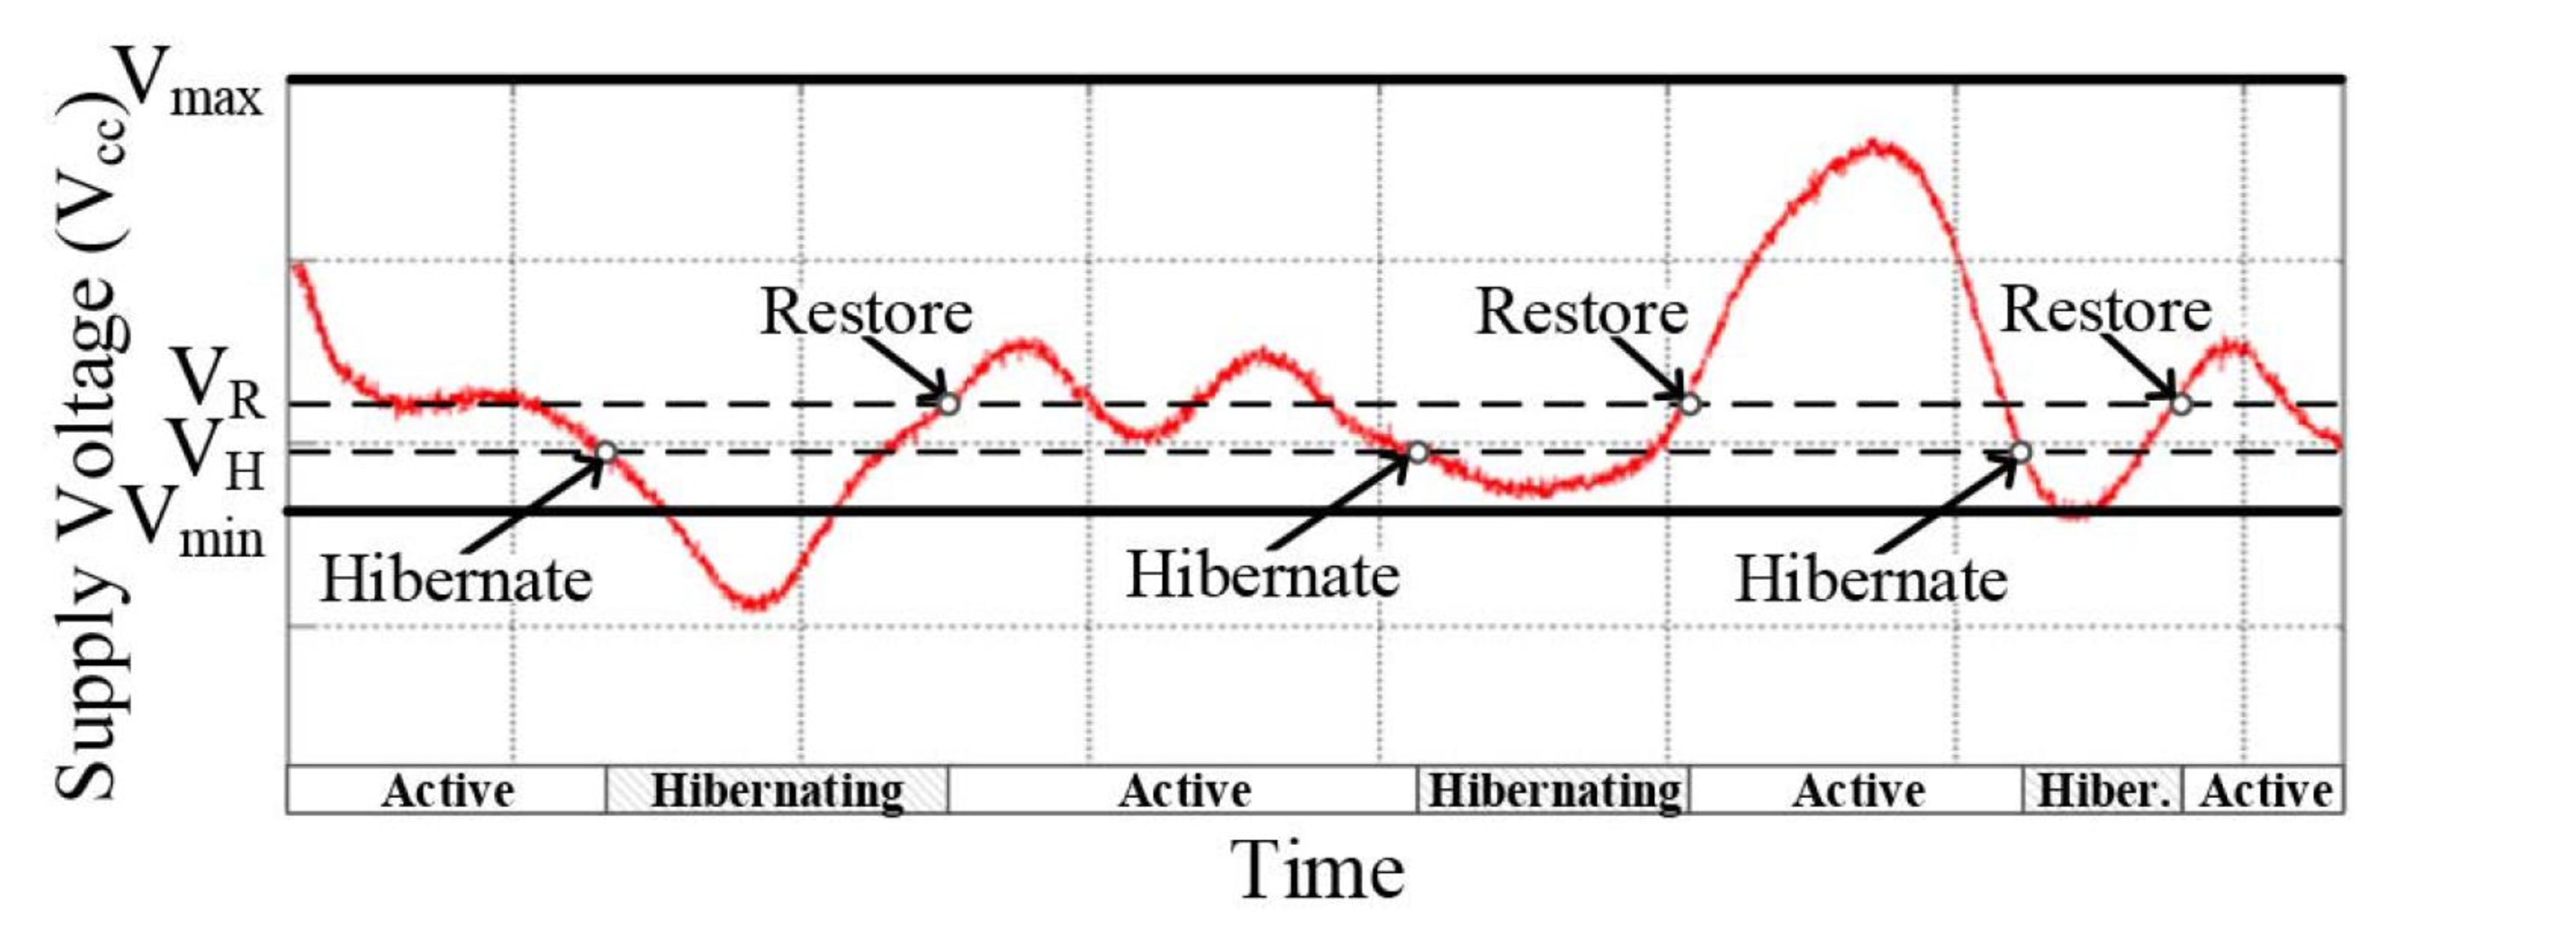
\includegraphics[width=14cm]{ch2_review/figures/hibernus}
    \caption{Voltage trace with hibernation and restoration points in Hibernus (taken from \cite{balsamo2015hibernus}).}
    \label{Figure:hibernus}
\end{figure}

Quickrecall~\cite{jayakumar2014quickrecall} is a similar approach to Hibernus except replacing RAM with NVM, so that all the run-time volatile data become non-volatile and only registers are necessary to be saved in a snapshot. An external voltage comparator detects a triggering voltage $V_{trig}$ to back up only peripherals and registers. Compared to the voltage thresholds in Mementos and Hibernus, $V_{trig}$ in Quickrecall is lower since the reduced energy and time overheads for saving and restoring a snapshot. However, using NVM as RAM may lead to the higher cost of NVM accesses. A comparison between Hibernus and Quickrecall is presented in~\cite{rodriguez2015approaches}, showing that Quickrecall performs worse when the frequency of power interrupts is low as the NVM consumes more than volatile RAM, and performs better when the frequency of power interrupts is high as the overheads of saving snapshots are much lower.

Reactive IC methods only save snapshots when power failure is imminent, and hence, reduce the number of snapshots compared to checkpointing methods. Also, reactive IC avoids code re-execution by suspending execution after saving a snapshot, and hence, ensures idempotency. 

% the size effect of energy buffers on reactive IC
The RAM usage varies at run time, so the size of snapshots in reactive IC also varies throughout code execution. To circumvent this issue, Hibernus saves the entire RAM in each snapshot while Quickrecall does not use RAM at all. Comparing Hibernus to checkpointing methods, the overheads of saving snapshots in Hibernus is larger as checkpointing methods can avoid saving large snapshots by analysing the program. Such high saving overheads becomes significant when the frequency of power outages increases. Increasing the size of energy storage in reactive IC should be helpful to mitigate frequent snapshot taking because the increased energy storage can filter the variations of supply voltage and avoid frequent voltage drops. 

\subsection{Harvest-Store-Use IC}

Harvest-store-use IC systems perform a complete task in one consecutive period when the harvested energy in energy storage is enough. A complete task typically includes sensing, processing, and transmitting actions. In order to sustain a successful task execution, the required capacity of energy storage is larger than the minimum required storage in other IC methodologies. Harvest-store-use systems need to calibrate the energy consumption of the task at design time and set an energy threshold to trigger execution based on that energy consumption. When the threshold is reached, which means there is enough energy for a task, the system performs one task and sleeps until the next threshold trigger. As shown in~\fref{Figure:saveanduse}, the behaviours of the amount of stored energy can be seen as alternating in turn between two states: the collecting state and the executing state.
% These systems work during the sporadic energy bursts.

\begin{figure}[!htb]
    \centering
    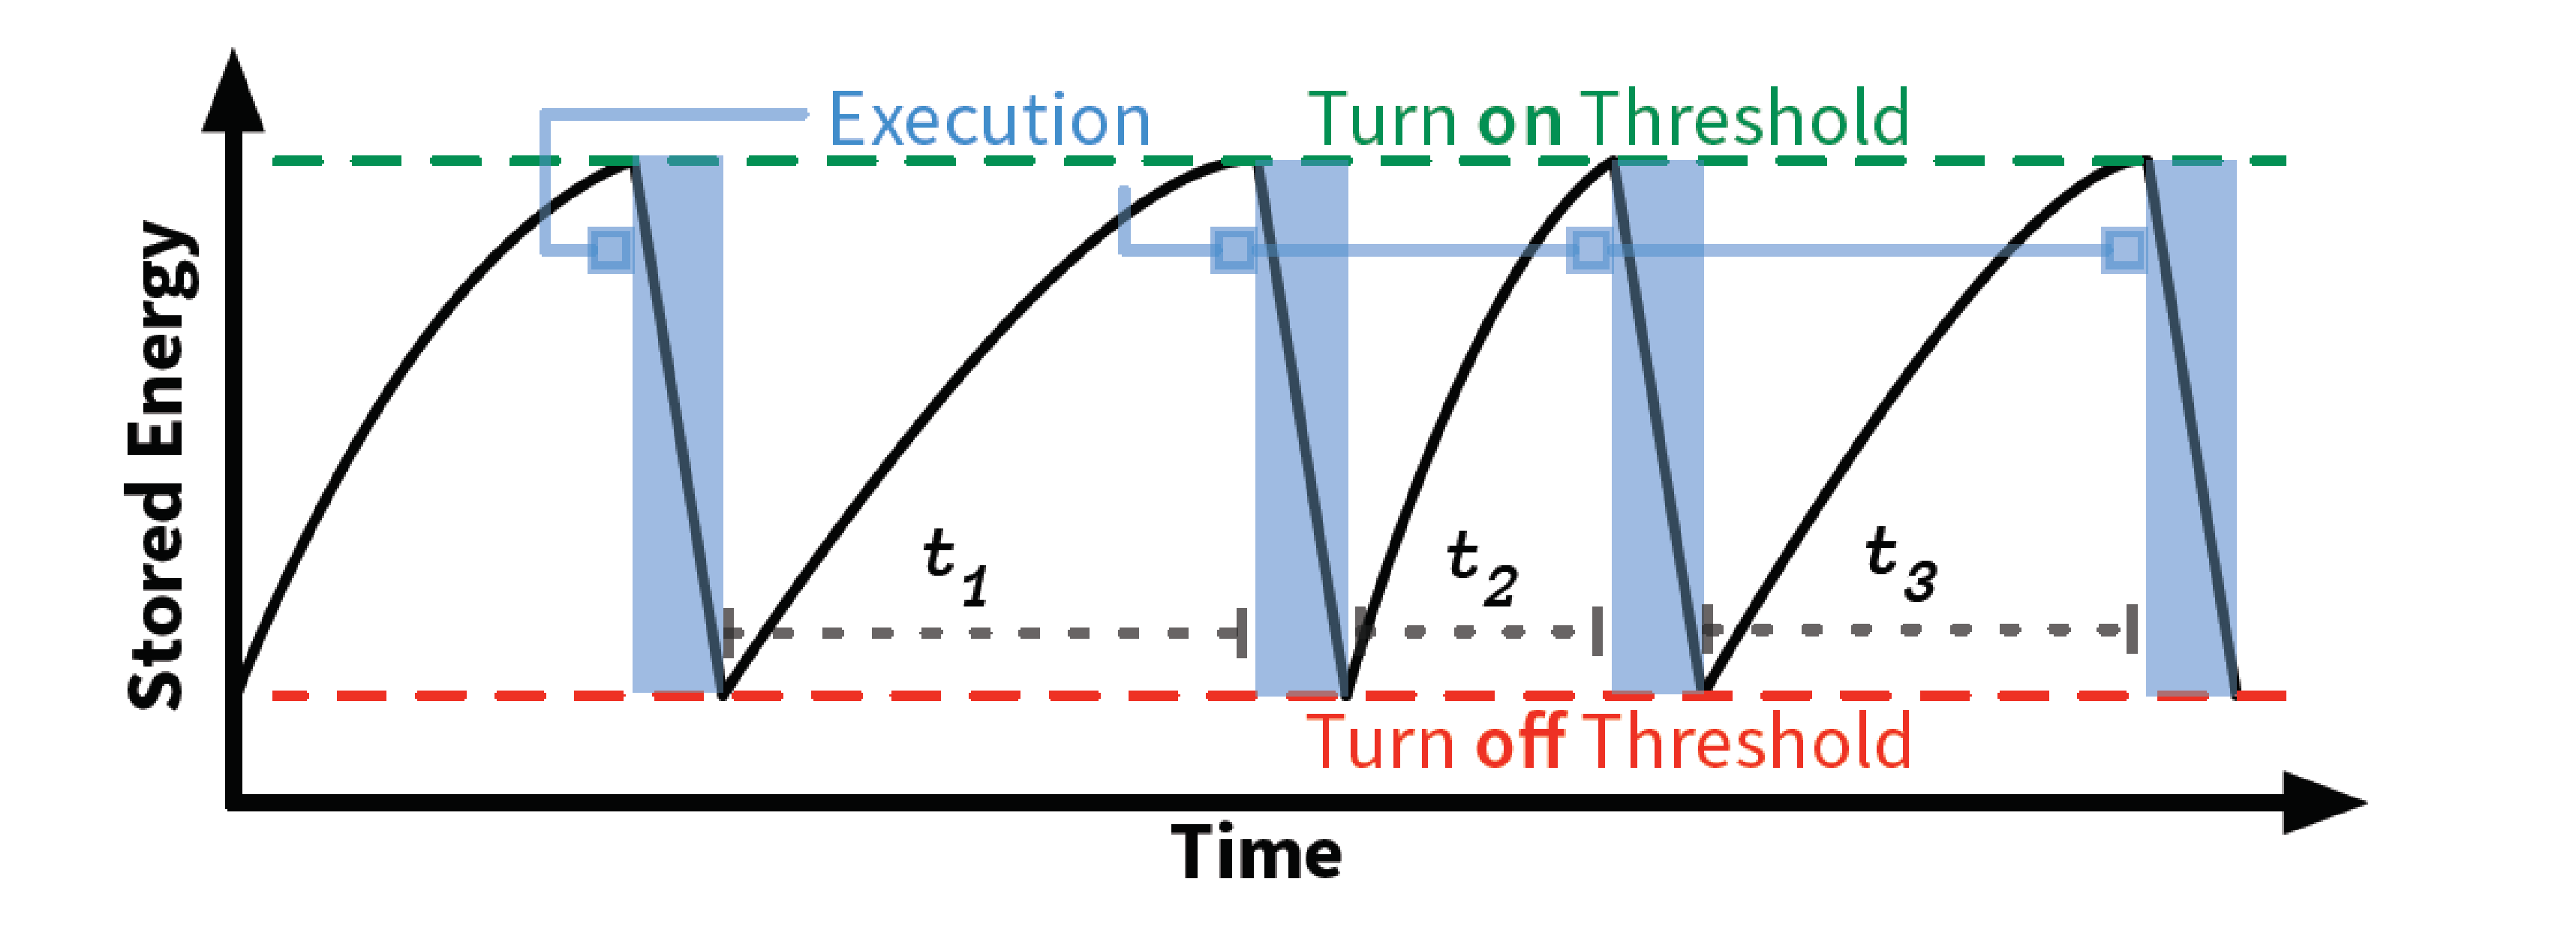
\includegraphics[width=14cm]{ch2_review/figures/saveanduse}
    \caption{Harvest-Store-Use execution (taken from~\cite{hester2017new}).}
    \label{Figure:saveanduse}
\end{figure}

Monjolo~\cite{debruin2013monjolo} is an early design following the harvest-store-use pattern. Monjolo presents a home power meter, whereby a current transformer is installed around the main power cable and provides the energy for this metering system. When the energy stored in a 500$\mu$F capacitor reaches a predefined amount, the system transmits a data packet. Another wireless receiver keeps collecting these packets and approximates the power of the main cable based on the receiving frequency of packets. Such a system contains little sensing and processing work on the transmitting node, and instead, it treats the intensity of energy sources as the sensing data, and processes this translation of data on the receiving node which is powered stably.

WISPCam~\cite{naderiparizi2015wispcam} is a wireless camera that obtains energy from an RF harvester. The harvested energy is stored in a 6mF supercapacitor and the data (photos) are saved in NVM. Once the energy is sufficient for taking one photo, the system starts execution and depletes the energy for taking a picture and data transmission. 

Similarly, Dynamic Energy Burst Scaling (DEBS)~\cite{gomez2016dynamic} also wakes up and executes tasks when there is enough energy in the 80$\mu$F capacitor. The major difference between DEBS and the above two approaches is DEBS can adjust the energy thresholds dynamically for a set of different tasks and generates energy bursts according to which task is in need.

Harvest-store-use paradigms are suitable for occasions where the harvested power is too weak to support the power consumption of any normal execution (other IC methodologies may quickly deplete energy storage and make little progress). Also, harvest-store-use methods circumvent the idempotency issues by complete tasks in one burst. However, this pattern is task-based, which means its operation is limited to one or several fixed energy-defined tasks and also relies on high-quality design-time profiling of tasks.

\subsection{Task-based IC}

% a figure to illustrate task-based IC?
Task-based IC decomposes a program into a series of atomic tasks, which only deliver non-volatile results after all operations in a task are completed~\cite{lucia2015simpler}. Task-based IC is achieved by programming and execution models, which aim to ensure NVM consistency and idempotency. In such models, accesses to NVM and I/O operations are carefully managed to prevent idempotent violations. To ensure idempotency, the program control flow is divided by task boundaries, and the communication between tasks is enabled by reading or writing NVM data on those boundaries. To avoid non-termination, the maximum size of one task is limited by the capacity of energy storage. Therefore, task-based IC can be seen as a rigorously-organized and fine-grained checkpointing method, which eliminates the the non-termination and idempotency problems in checkpointing IC. Task-based systems feature with fast suspend and restore operations because only the runtime and the current task should be versioned and restored through power outages~\cite{sliper2018enabling}. 

DINO~\cite{lucia2015simpler} proposes the first task-based IC programming and execution model, illustrating the task-based idea and providing a basic groundwork. DINO implements the programming and execution model on the LLVM compiler for C code, with program libraries and compiler passes. Chain~\cite{colin2016chain} improves DINO data flows with "Channels", which is dedicated to manage non-volatile data, guaranteeing the correctness on applications with both idempotent and non-idempotent code. Alpaca~\cite{maeng2017alpaca} introduces data privatization which reduces memory usage compared to Chain.

A main drawback of DINO, Chain, and Alpaca is they require great programming efforts for programmers to understand the implemented libraries and redesign a program according to the task-based concept. A recent work, CleanCut~\cite{colin2018termination}, proposes an auxiliary tool to check and automatically decompose the non-terminating tasks (the energy consumption of which exceeds the capacity of system energy storage). 

Also, like checkpointing IC, task-based IC inevitably involves re-execution. Alpaca, the state-of-the-art task-based approach, reports a run time overhead of 1.3-3.6x compared to plain C code given constant power supply. 

\subsection{Non-Volatile Processors}

Non-Volatile Processors (NVPs) incorporate automatic backup and restore hardware within the chips. A comparison of memory architecture between traditional processors and NVPs is shown in~\fref{Figure:nvp}. The traditional volatile elements are replaced with non-volatile elements to achieve efficient backup and restore operations with a faster speed and lower energy consumption than the conventional memory architecture. To be specific, the registers and cache are equipped with built-in additional non-volatile backup and restore circuits, so that when the supply power is going to disappear, the computing state can be saved locally just beside the elements, rather than being copied out into an external NVM. It is reported that the backup and restore speed of NVPs can be 2-4$\times$ magnitudes faster than the state-of-the-art NVM based commercial processors~\cite{liu2015ambient}. 

\begin{figure}[!htb]
    \centering
    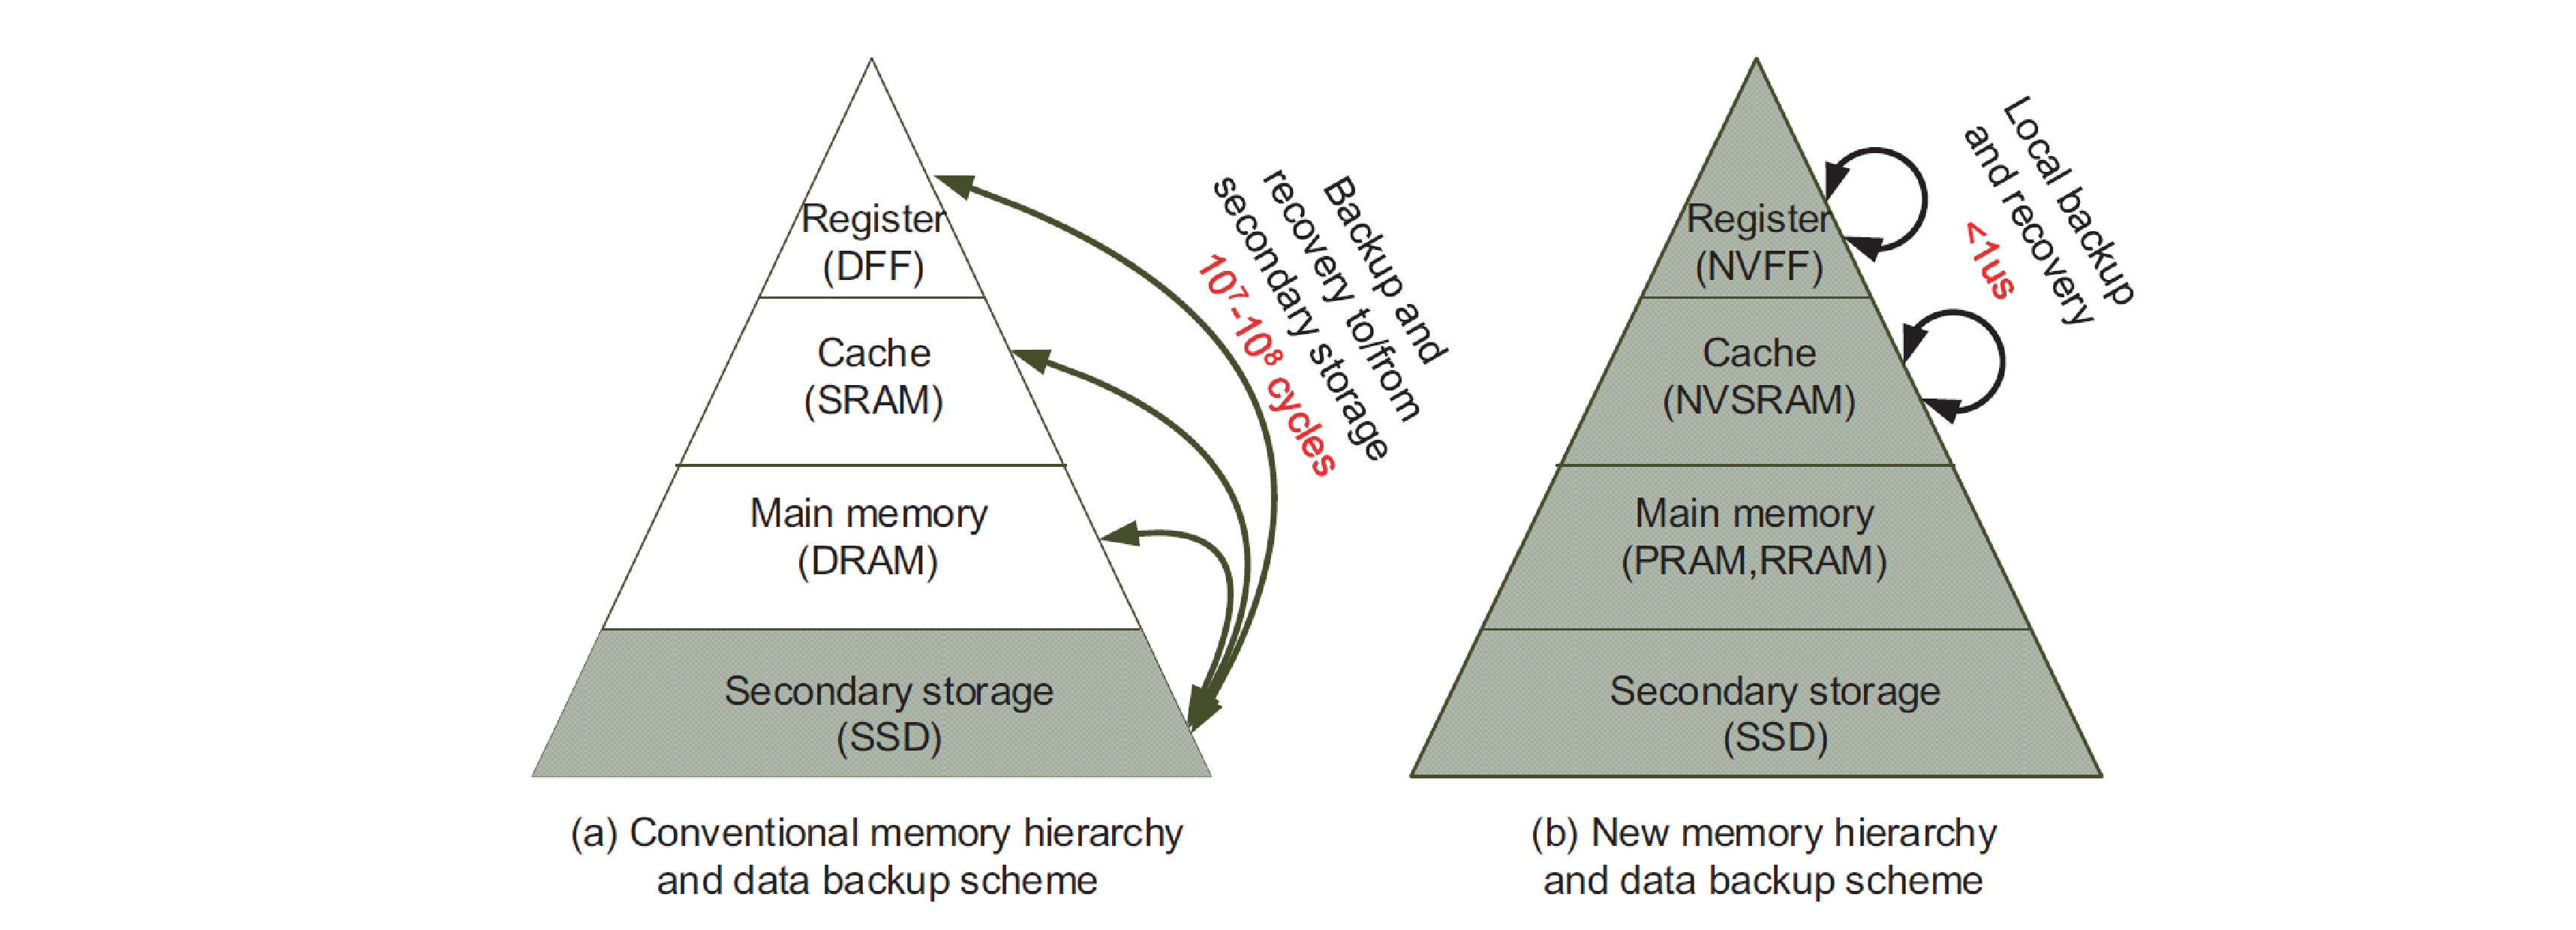
\includegraphics[width=12cm]{ch2_review/figures/nvp}
    \caption{Memory architectures of traditional processors and NVPs (taken from~\cite{liu2015ambient}).}
    \label{Figure:nvp}
\end{figure}

Wang \textit{et al.}~\cite{wang20123us} present a preliminary NVP with 3$\mu$s backup time and 7$\mu$s restore time, which enables the processor to operate safely under a 20 kHz square wave of power. As a comparison, the existing MCUs in TI MSP430 family can only achieve 212$\mu$s and 310$\mu$s for saving and restoring states respectively. Su \textit{et al.}~\cite{su2017ferroelectric} extend the backup and restore time overheads to a system level, presenting a NVP with 46$\mu$s system-level wake-up time and 14$\mu$s system-level sleep time. Liu \textit{et al.}~\cite{liu2019130} integrate a NVP into a system-on-chip with independent backup and restore circuits for peripherals. 

NVP-based research follows with the development of NVP hardware. Ma \textit{et al.}~\cite{ma2015architecture} examine the performance and energy consumption of several types of NVPs with different ambient sources, providing a guideline for NVPs selection. The concept of "Incidental Computing" based on NVPs is proposed in~\cite{ma2017incidental} to improve the forward progress under unstable power supply, and also provides an evaluation of performance on NVPs. Essentially, it pays more attention to processing forward data in need than the buffered historical data from recovery, but an incidental recomputing on the historical data is performed when there is abundant energy. It is reported that this approach outperforms the existing save-and-use computing scheme by 2.2-5$\times$ in the simulation with respect to an image processing speed, and also the forward progress is improved by 4.28$\times$ on average over a basic NVP.

NVPs perform well in terms of the response to power intermittency, but the research on how to deliver better forward progress with NVPs is limited. Dynamic Voltage and Frequency Scaling (DVFS) can be a potentially applicable solution~\cite{ma2016nonvolatile}. In a traditional NVP, the small buffering capacitor tends to be either charged to be full or depleted rapidly and frequently~\cite{su2017nonvolatile}. This behaviour accounts for a large part of backup and recovery overheads, so power management based on NVP is in need.

\section{Power-Neutral Computing} \label{Section:PN}

While IC aims to ensure forward execution despite frequent power outages, energy harvesters may also generate more power than systems can consume when ambient sources are sufficient. Such excessive energy is wasted if not stored for later usage or consumed immediately. 
% Adaptive computing in energy harvesting computing denotes energy management techniques that aim to efficiently utilise the harvested energy. 
% Different sizes of storage supports different scale of energy management.

\subsection{Principles of Operations}

Power-neutral (PN) computing aims to manage power without additional storage or with only a very limited amount of storage which can only sustain its system for milliseconds. In principle, power-neutral computing is a special case of energy neutral computing when $\Delta t$ in Equation~\ref{eq:energyneutral} is equal (or close) to zero. Technically, PN computing scales the instantaneous system power consumption to match the instantaneous harvested power with theoretically zero storage (in other words, energy neutrality is met instantaneously). PN operations can be translated into the following expressions:

\begin{equation} \label{eq:pn}
    P_h(t) = P_c(t)
\end{equation}
\begin{equation} \label{eq:pnon}
    where\quad t \in \{t|V_{cc}(t) \geq V_{min}\}
\end{equation}

where $V_{cc}$ is the input voltage of the computing load, and $V_{min}$ is the minimum voltage required for the system to operate. Equation~\ref{eq:pn} describes the methodology of power neutrality (dynamic and instantaneous power adaptation). Equation~\ref{eq:pnon} limits the requirement for power neutrality that the system should be powered and active to make reactions of performance scaling. This requirement may change according to different system designs, but for contemporary computing and sensing loads, this is determined by the supply voltage. 

Given a very limited amount of storage and a range of scalable performance and power consumption, PN computing scales down performance if $P_h$ is lower than $P_c$, such that $V_{cc}$ remains stable, which extends execution time and avoids suspend and restore operations. On the other hand, PN computing scales up performance if $P_h$ is higher than $P_c$, such that the excessive harvested energy is immediately consumed on useful work rather than wasted.

In practice, however, there does not exist a system that can adjust its power consumption instantaneously to the harvested power without any overheads. Any performance scaling costs a small amount of time and energy overheads, which a system cannot afford without any energy storage. Therefore, a minimum storage is still required, normally in the form of decoupling or parasitic capacitance, to provide a small but sufficient amount of energy for scaling performance and adapting power consumption.
% In practice, a PN system tries to meet Equation~\ref{eq:pn} as quickly as possible while switching overheads still exist.
% switching granularity/resolution?

In order to achieve power neutrality, a system has to adapt its performance and hence power consumption. Performance scaling can be achieved by hardware controlling, such as Dynamic Frequency Scaling (DFS)~\cite{balsamo2016graceful}, Dynamic Voltage and Frequency Scaling (DVFS)~\cite{fletcher2017power}, or switching on/off load elements~\cite{wang2016storage, fletcher2017power} (also known as Dynamic Power Management, DPM~\cite{lu2000low} or hot-plugging). Apart from these achieved methods, duty-cycle scaling and task scheduling are also choices for changing performance and consumption, though they have not been implemented in current research yet.

\subsection{Recent Approaches}

The concept of PN computing is proposed in~\cite{balsamo2016graceful} and implemented on a Texas Instrument MSP430FR5739 MCU without an external energy buffer. As shown in~\fref{Figure:graceful_schematic}, the executing load is directly connected to a regulated energy harvesting source. The control scheme in~\cite{balsamo2016graceful} utilises DFS with a voltage feedback. Specifically, two voltage thresholds, $V_{dec}$ and $V_{inc}$, are set for detecting voltage variance caused by power inequality and then scaling performance accordingly. In order to respond fast to power difference, the capacitance is reduced to 19$\mu$F, which is only the parasitic and on-board decoupling capacitance. When $P_h(t) > P_c(t)$ and the operating voltage $V_{cc}$ increases rapidly due to the small capacitance and reaches $V_{inc}$, the MCU increases its operating frequency resulting in faster computing speed and higher power consumption, and also increases the thresholds between which the new voltage value is contained; and vice versa, a reverse procedure is executed for $P_h(t) < P_c(t)$. In a word, this control scheme is trying to make the operating voltage stable around a desired value so that $P_h(t)$  equals $P_c(t)$ approximately.

\begin{figure}[!htb]
    \centering
    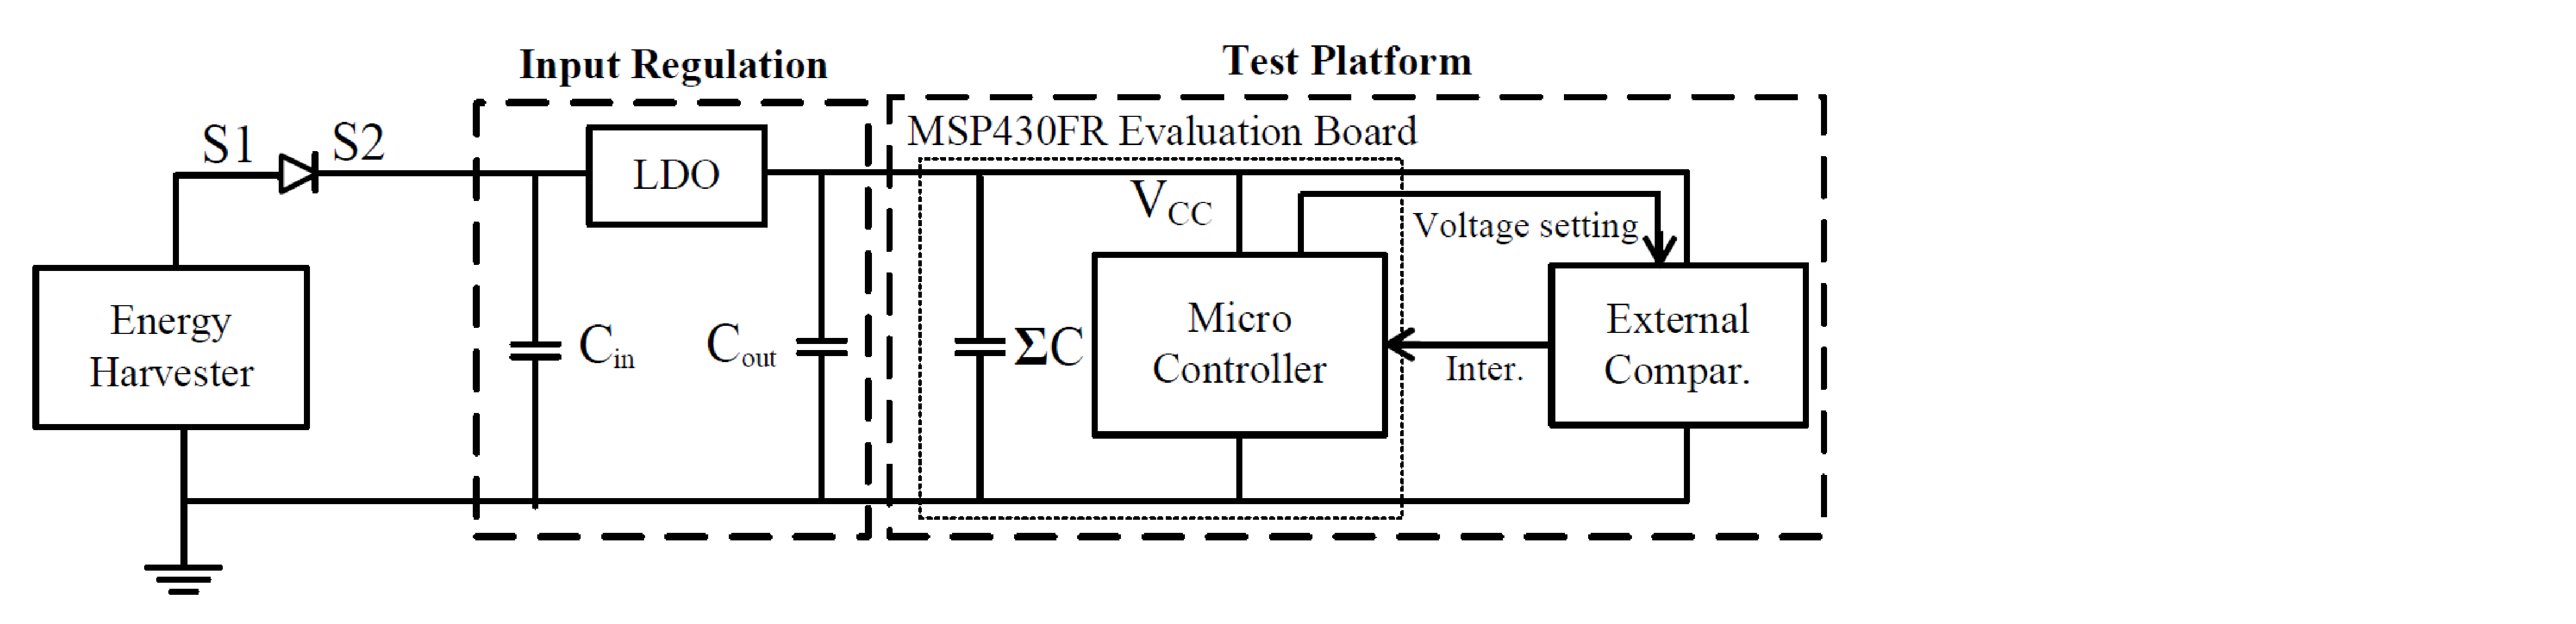
\includegraphics[width=14cm]{ch2_review/figures/graceful_schematic}
    \caption{Architecture of an example power neutral system based on TI MSP430FR platform (taken from \cite{balsamo2016graceful}).}
    \label{Figure:graceful_schematic}
\end{figure}
%flowchart of this control scheme is present in figure?

A similar control scheme is adopted in~\cite{fletcher2017power} where the platform is an MP-SoC adopting DVFS and DPM, which leads to higher performance, higher power consumption, and more operating points than the MCU in~\cite{balsamo2016graceful}. A 47mF supercapacitor is used for safely overcoming performance switching where the power consumption of the board is normally above 2W. As an illustration for how to scale performance by DVFS and DPM, \fref{Figure:dvfs} presents an example application profile of 'power consumption vs performance' when DVFS and DPM applied on a heterogeneous multi-processor system-on-chip (MP-SoC) platform. The SoC used in this platform is the Samsung Exynos5422 big.LITTLE SoC with four 'big' high-performance A15 cores and four 'LITTLE' low-power A7 cores. In this case, the performance refers to the speed of executing this application for one time and is proportional to the operating frequency under a certain core configuration. As shown in the figure, each performance level (a pair of frequency and core status, also named as an operating point) requires a certain power consumption. At run-time, the system dynamically switch its performance among these operating points so as to timely match $P_c(t)$ with $P_h(t)$.

\begin{figure}[!htb]
    \centering
    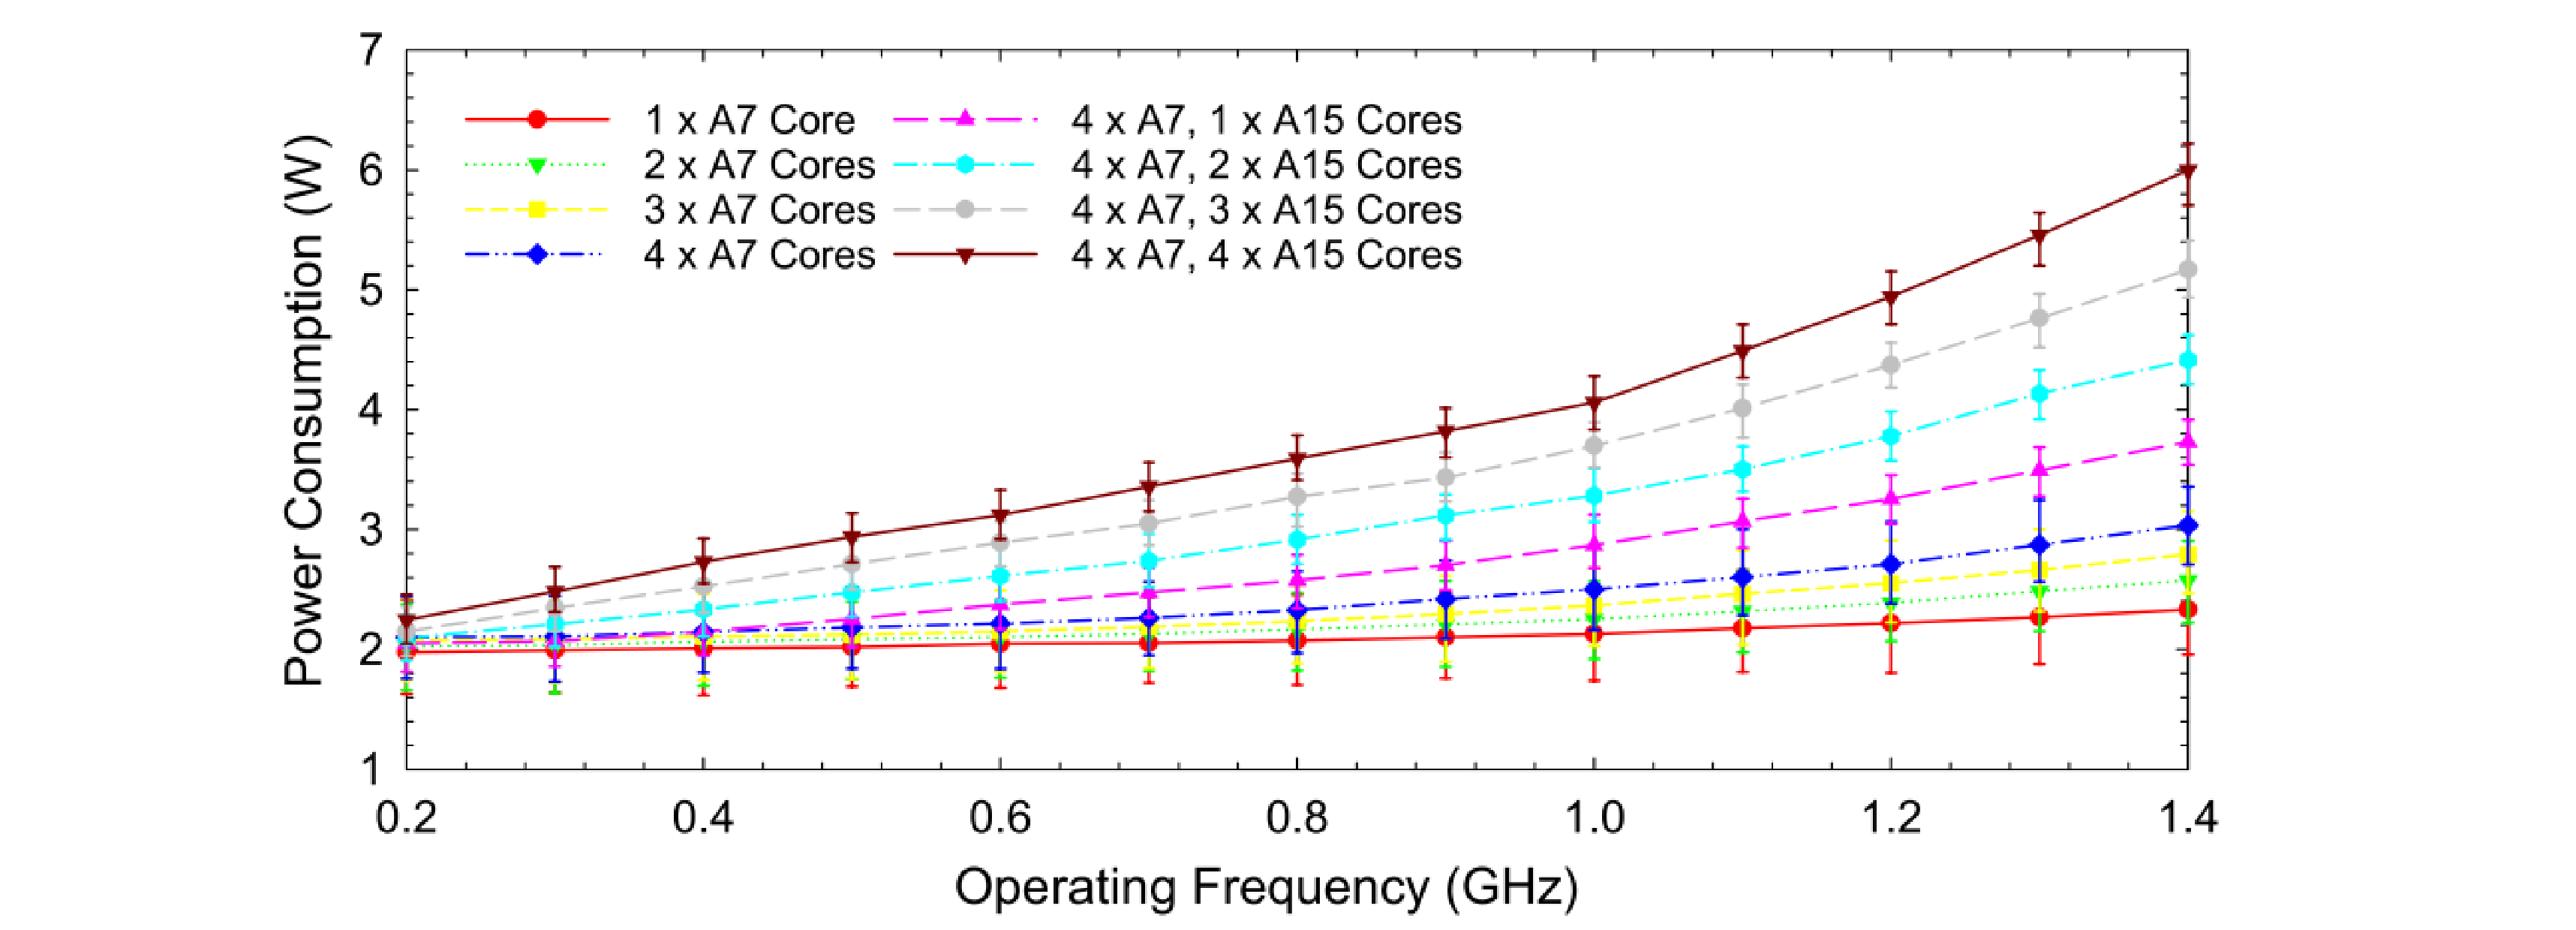
\includegraphics[width=14cm]{ch2_review/figures/dvfs}
    \caption{Board power consumption of ODROID XU4 vs operating frequency and core configurations, running CPU intensive application Raytrace (taken from \cite{fletcher2017power}).}
    \label{Figure:dvfs}
\end{figure}

There are three advantages in this kind of PN control scheme. First, the voltage is stabilized so it can offset ephemeral power drops which cause insufficient voltage supply and power failures, and therefore the lifetime increases (e.g. reported by 4-88\% in~\cite{balsamo2016graceful}). Second, as power neutral computing eliminates many elements that required in EN systems, such as large energy storage, power converters and MPPT units, the size and cost of devices is reduced and the number of power consumption components also decreases. Third, if powered by a solar panel and the operating voltage range encompasses the MPP of the given solar panel, the system embraces an intrinsic MPPT characteristic as it can stabilize the voltage around a target value.

Similarly, Wang \textit{et al.}~\cite{wang2016storage} propose a storage-less and converter-less approach which can be classified as a power neutral system. In this design, a 47$\mu$F bulk capacitor is equipped with a 3.29mW non-volatile MCU and up to 16.5mW peripherals. This capacitor is also small enough compared to the 19$\mu$F capacitance operating with an up to 3 mW MCU in~\cite{balsamo2016graceful}. An external MPPT controlling element dynamically adjusts the power duty-cycle for the non-volatile load in order to match the harvested current and the consumed current, and hence power neutrality is met. 

One disadvantage of power neutral computing is that it has to passively scale its power consumption as well as its performance, causing large variations in performance. However, this might not be good in terms of the overall forward progress. In the next chapter, a preliminary analyse is explained about how the forward progress is improved when the capacitor size is increased, while not violating the merits of PN computing. 

\section{Summary}

This chapter introduces a background of energy harvesting techniques, summarises the evolution of energy storage used in energy harvesting computing, and reviews the existing methodologies of battery-less energy harvesting computing. 

EN computing emphasizes the continuous activity of devices over a long-term duration (e.g. several days, one year) by buffering harvested energy in large energy storage and adapting energy consumption "reluctantly". However, large energy buffers, usually in the form of batteries or large supercapacitors, are demanded for EN operations, whereas such large energy storage limits device lifespans, increases the cost, mass, dimensions of devices, and bring pollution and maintenance issues. This contradicts the design requirements of ubiquitous sensor deployments. 
% Besides, EN operations rely heavily on a predictable power source otherwise it is hard to identify how much energy is required and how long such energy should be balanced for. 

To circumvent the limitations in EN computing, intermittent computing is recently developed. Intermittent computing continues computation after the supply fails rather than restarts from the beginning of programs. Hence, intermittent computing devices can achieve forward execution despite frequent power failures with only minimum storage (e.g. a decoupling capacitor) to secure successful saving and restoring operations of computing states between volatile and non-volatile components. Based on intermittent computing, PN computing introduces run-time performance adaptation to match power consumption with harvested power, such that the number of saving and restoring operations can be reduced and application execution speed is increased. 

However, with minimised storage, an intermittent computing device has to frequently wake up, execute shortly, and halt when the harvested power is less than the load power consumption, consuming much energy in managing system states. As for PN computing, volatile power from environment results in significant performance variations, which then cause performance loss. The remaining part of this thesis reports a study on how to mitigate these two problems and improve system execution speed by adding a small amount of energy storage without significantly affect device dimensions. 
